\documentclass[11pt, a4paper]{article}

% --- PREAMBLE ---
% Set up packages for math, code, graphics, and layout
\usepackage[utf8]{inputenc}
\usepackage[T1]{fontenc}
\usepackage{lmodern}
\usepackage[margin=1.5in]{geometry}
\usepackage{amsmath}
\usepackage{amssymb}
\usepackage{graphicx}
\usepackage{hyperref}
\usepackage{xcolor}
\usepackage{listings}
\usepackage{palatino} % Use a more "textbook-like" font
\usepackage{mathpazo} % Use Palatino-compatible math fonts
\usepackage{microtype} % Improves text justification and reduces overfull boxes
\usepackage{tikz}
\usepackage{enumitem}
\usepackage{float}
\setlength{\parindent}{0pt}
% \setlength{\parskip}{1em}
\setlist[itemize]{noitemsep, topsep=0pt}

% Define colors for code listings
\definecolor{codegreen}{rgb}{0,0.6,0}
\definecolor{codegray}{rgb}{0.5,0.5,0.5}
\definecolor{codepurple}{rgb}{0.58,0,0.82}
\definecolor{backcolour}{rgb}{0.95,0.95,0.95}

% Configure the 'listings' package for Python
\lstdefinestyle{mystyle}{
    backgroundcolor=\color{backcolour},   
    commentstyle=\color{codegreen},
    keywordstyle=\color{magenta},
    numberstyle=\tiny\color{codegray},
    stringstyle=\color{codepurple},
    basicstyle=\ttfamily\footnotesize,
    breakatwhitespace=false,         
    breaklines=true,                 
    captionpos=b,                    
    keepspaces=true,                 
    numbers=left,                    
    numbersep=5pt,                  
    showspaces=false,                
    showstringspaces=false,
    showtabs=false,                  
    tabsize=4,
    language=Python,
    morecomment=[l]{\#},
}
\lstset{style=mystyle}

% Allow line breaks in inline \texttt{} commands at underscores and other characters
\usepackage{xspace}
\usetikzlibrary{shapes,arrows,positioning,shadows,fit,decorations.pathreplacing,backgrounds}

% Improve hyphenation and line breaking - balanced settings
\tolerance=2000
\emergencystretch=3em
\hfuzz=0.5pt

% Setup for the title page
\title{Programming Techniques for Scientific Simulations I: \\ A Comprehensive Introduction to Python and C++}
\author{Based on lecture slides}
\date{\today}

% Hyperlink setup
\hypersetup{
    colorlinks=true,
    linkcolor=blue,
    filecolor=magenta,      
    urlcolor=cyan,
    pdftitle={Programming Techniques for Scientific Simulations},
    pdfpagemode=FullScreen,
}

\begin{document}

\maketitle
\tableofcontents
\newpage

% ============================================================================
% PART I: PYTHON SCIENTIFIC COMPUTING
% ============================================================================

\section{Introduction to Advanced Python for Scientific Computing}

This chapter provides a comprehensive exploration of Python's scientific computing ecosystem, focusing on the fundamental libraries that form the foundation of computational science: NumPy, SciPy, and Matplotlib. These tools have become the de facto standards for numerical computing in Python, offering both high performance and ease of use. We will also explore essential practices for managing Python environments and dependencies, ensuring reproducible computational workflows.

Scientific computing requires not only mathematical sophistication but also robust software engineering practices. Python's ecosystem has evolved to meet these demands through carefully designed libraries that balance performance with accessibility. The journey begins with understanding how to create isolated, reproducible computing environments, then progresses through array computing, mathematical operations, and visualization techniques essential for modern computational science.

\subsection{The Importance of Environment Management}

Before diving into numerical computing, we must understand how to manage Python environments properly. In professional scientific computing, different projects often require different versions of libraries, and changes in one project should never affect another. This is where virtual environments become essential.

\section{Python Virtual Environments (venv)}

\subsection{Understanding Virtual Environments}

A \textbf{virtual environment (venv)} is a lightweight, self-contained Python environment that includes its own Python interpreter and a separate set of installed packages. Think of it as creating a isolated "bubble" for each of your projects, where the dependencies and package versions are completely independent from your system Python installation and from other projects.

\textbf{Why is this important?} Imagine you are working on two scientific projects simultaneously. Project A requires NumPy version 1.19 for compatibility with legacy code, while Project B needs NumPy version 1.24 to use new features. Without virtual environments, you would be forced to install only one version system-wide, breaking one of your projects. Virtual environments solve this problem elegantly by allowing each project to maintain its own dependency versions.

\subsection{Key Benefits of Using Virtual Environments}

\begin{itemize}
\item \textbf{Isolated Environment Per Project}: Each project has its own independent Python environment. Installing, upgrading, or removing packages in one environment has absolutely no effect on other environments or the system Python.

\item \textbf{Prevention of Version Conflicts}: Different projects can require different versions of the same library without conflict. This is critical in scientific computing where reproducibility often depends on specific package versions.

\item \textbf{Reproducibility and Collaboration}: Virtual environments make it easy to document and share the exact dependencies needed for a project. Collaborators can recreate your environment precisely, ensuring that code runs identically across different machines.

\item \textbf{Clean System Python}: Your system Python installation remains pristine and uncluttered. This is particularly important on Linux systems where system tools may depend on specific Python package versions.
\end{itemize}

\subsection{Creating and Managing Virtual Environments}

\subsubsection{Creating a Virtual Environment}

The process of creating a virtual environment is straightforward but follows a specific pattern. You use Python's built-in \texttt{venv} module to create a new directory that will contain the isolated environment.

\textbf{Syntax:}
\begin{lstlisting}[language=bash]
python -m venv name_of_your_environment
\end{lstlisting}

\textbf{Component Breakdown:}
\begin{enumerate}
\item \texttt{python}: Invokes the Python interpreter
\item \texttt{-m venv}: Executes the venv module as a script
\item \texttt{name\_of\_your\_environment}: The directory name where the virtual environment will be created (commonly named \texttt{venv}, \texttt{env}, or something project-specific like \texttt{myproject\_env})
\end{enumerate}

When this command executes, Python creates a new directory structure containing:
\begin{itemize}
\item A copy of the Python interpreter
\item Standard library links
\item A \texttt{site-packages} directory for installed packages
\item Activation scripts for different shells
\item Configuration files
\end{itemize}

\subsubsection{Activating the Virtual Environment}

Creating the environment is only the first step; you must \textbf{activate} it to use it. Activation modifies your shell's environment variables so that when you run \texttt{python} or \texttt{pip}, it uses the versions from your virtual environment rather than the system versions.

\textbf{Linux / macOS Activation:}
\begin{lstlisting}[language=bash]
. name_of_your_environment/bin/activate
# or equivalently:
source name_of_your_environment/bin/activate
\end{lstlisting}

\textbf{Windows PowerShell Activation:}
\begin{lstlisting}[language=bash]
.\name_of_your_environment\Scripts\Activate.ps1
\end{lstlisting}

After activation, you will typically see the environment name in parentheses in your shell prompt, indicating that the environment is active, for example:
\texttt{(name\_of\_your\_environment) user@machine:\~\$}

\subsubsection{Installing Packages in the Virtual Environment}

Once activated, you can install packages using \texttt{pip}, and they will be installed only in this virtual environment:

\begin{lstlisting}[language=bash]
pip install numpy scipy matplotlib h5py
\end{lstlisting}

This command installs multiple scientific computing packages simultaneously. Each package is downloaded and installed into the virtual environment's \texttt{site-packages} directory.

\subsubsection{Deactivating the Virtual Environment}

When you finish working in a virtual environment, you should deactivate it to return to your normal shell environment:

\begin{lstlisting}[language=bash]
deactivate
\end{lstlisting}

This command is available once you've activated a virtual environment. It reverses the changes made during activation, restoring your original \texttt{PATH} and other environment variables.

\subsection{Ensuring Reproducibility with Requirements Files}

One of the most powerful features of Python's packaging ecosystem is the ability to precisely document and reproduce environments. This is accomplished through \textbf{requirements files}.

\subsubsection{Exporting Your Environment}

To create a snapshot of all packages currently installed in your environment, use:

\begin{lstlisting}[language=bash]
pip freeze > requirements.txt
\end{lstlisting}

This creates a \texttt{requirements.txt} file containing every installed package with its exact version number. The format looks like:
\begin{lstlisting}
numpy==1.24.3
scipy==1.10.1
matplotlib==3.7.1
h5py==3.8.0
\end{lstlisting}

The \texttt{==} notation specifies exact versions, ensuring complete reproducibility.

\subsubsection{Recreating an Environment}

Given a \texttt{requirements.txt} file (perhaps from a colleague or from a project repository), you can recreate the exact same environment:

\begin{lstlisting}[language=bash]
pip install -r requirements.txt
\end{lstlisting}

The \texttt{-r} flag tells pip to read the requirements from a file. This will install every package listed, at the exact versions specified, allowing anyone to recreate your computing environment precisely.

\subsubsection{Complete Workflow Example}

Here is a complete example of setting up a scientific computing project with a virtual environment:

\begin{lstlisting}[language=bash, caption={Complete virtual environment workflow}]
# 1. Create a new directory for your project
mkdir my_simulation_project
cd my_simulation_project

# 2. Create a virtual environment
python -m venv sim_env

# 3. Activate the environment
. sim_env/bin/activate

# 4. Install required packages
pip install numpy scipy matplotlib h5py

# 5. Document the environment
pip freeze > requirements.txt

# 6. Work on your project...
# (write code, run simulations, etc.)

# 7. When done, deactivate
deactivate
\end{lstlisting}

\textbf{Best Practices:}
\begin{itemize}
\item Always create a virtual environment for each project
\item Keep the \texttt{requirements.txt} file in version control (Git)
\item Update \texttt{requirements.txt} whenever you install new packages
\item Use descriptive environment names that indicate the project or purpose
\item Never commit the virtual environment directory itself to version control (it can be large and is machine-specific); only commit \texttt{requirements.txt}
\end{itemize}

\section{NumPy: The Foundation of Numerical Computing in Python}

\subsection{Introduction to NumPy}

\textbf{NumPy} (Numerical Python) is the fundamental package for scientific computing in Python. It is not an exaggeration to say that NumPy forms the foundation upon which the entire scientific Python ecosystem is built. Almost every scientific computing library in Python either depends on NumPy directly or follows its conventions.

\textbf{What does NumPy provide?} NumPy offers three critical capabilities:

\begin{enumerate}
\item \textbf{A powerful N-dimensional array object}: The \texttt{ndarray} is a fast, flexible container for large datasets in Python. Unlike Python lists, NumPy arrays are homogeneous (all elements have the same type) and stored in contiguous blocks of memory, enabling extremely efficient computation.

\item \textbf{A large collection of high-level mathematical functions}: NumPy provides mathematical functions that operate on entire arrays without the need for explicit loops. This is called \textbf{vectorization} and is key to writing efficient numerical code.

\item \textbf{Useful capabilities for linear algebra, Fourier transforms, and random number generation}: NumPy includes sophisticated functionality that forms the backbone of many scientific algorithms.
\end{enumerate}

\subsection{The Import Convention}

By convention, NumPy is imported with the alias \texttt{np}:

\begin{lstlisting}[language=Python]
import numpy as np
\end{lstlisting}

This convention is nearly universal in the Python scientific computing community. Using \texttt{np} makes code more concise while maintaining clarity about which functions come from NumPy.

\subsection{Why NumPy is Fast: A Performance Comparison}

To understand why NumPy is essential for scientific computing, consider a simple operation: squaring every element in a collection of 1000 numbers.

\textbf{Pure Python approach:}
\begin{lstlisting}[language=Python, caption={Pure Python list comprehension}]
a = range(1000)
result = [i**2 for i in a]
\end{lstlisting}

\textbf{NumPy approach:}
\begin{lstlisting}[language=Python, caption={NumPy vectorized operation}]
b = np.arange(1000)
result = b**2
\end{lstlisting}

The slides demonstrate using IPython's magic function \texttt{\%timeit} to compare performance:

\begin{lstlisting}[language=Python, caption={Performance comparison using IPython magic}]
In []: a = range(1000)
In []: %timeit [i**2 for i in a]
# Output shows timing, e.g., ~100 microseconds per loop

In []: b = np.arange(1000)
In []: %timeit b**2  
# Output shows timing, e.g., ~2 microseconds per loop
\end{lstlisting}

\textbf{Why is NumPy so much faster?} The performance difference (often 50-100x faster) comes from several factors:

\begin{itemize}
\item \textbf{Contiguous memory storage}: NumPy arrays store data in contiguous blocks of memory, enabling efficient cache utilization by the CPU.

\item \textbf{Vectorized operations in C}: NumPy's operations are implemented in highly optimized C code that avoids Python's interpreter overhead.

\item \textbf{No Python loop overhead}: The Python list comprehension must call Python's interpreter for each element. NumPy performs the entire operation in compiled code.

\item \textbf{Type homogeneity}: Because all elements in a NumPy array are the same type, the operation can be optimized without type checking at each step.
\end{itemize}

\textbf{Note on IPython Magic Functions}: IPython provides special commands called "magic functions" that start with \texttt{\%}. The \texttt{\%timeit} magic function automatically runs code multiple times and reports the best timing, which is useful for benchmarking. These magic functions only work in IPython or Jupyter environments, not in regular Python scripts.

\subsection{Documentation and Resources}

NumPy has excellent, comprehensive documentation available at \url{https://numpy.org/}. The documentation includes:
\begin{itemize}
\item User guide with tutorials for beginners
\item Complete API reference for all functions
\item Detailed explanations of array operations and broadcasting rules
\item Performance tips and best practices
\end{itemize}

\section{NumPy Basics: Understanding the ndarray}

\subsection{The ndarray Object}

The \texttt{ndarray} (N-dimensional array) is NumPy's fundamental data structure. Understanding this object is crucial for effective scientific computing in Python.

\subsubsection{Key Characteristics of ndarray}

\textbf{Homogeneity}: An ndarray is a container of items of the \textbf{same type}. You cannot mix integers and strings in the same array, unlike Python lists. This restriction is not a limitation but rather a feature that enables performance and memory efficiency.

\textbf{Multi-dimensional}: Arrays can have any number of dimensions (axes). Common cases:
\begin{itemize}
\item 1D array: A vector, similar to a list
\item 2D array: A matrix or table of data
\item 3D array: A volume or stack of matrices (common in image processing)
\item Higher dimensions: Commonly used in machine learning and scientific simulations
\end{itemize}

\textbf{Indexing}: Arrays are indexed by tuples of positive integers, using \textbf{zero-based indexing} just like C/C++. This differs from mathematical conventions (which often start at 1) but is standard in computer science.

\subsubsection{Creating Your First Array}

\begin{lstlisting}[language=Python, caption={Creating a simple 2D array}]
import numpy as np

# Create a 2D array (2 rows, 3 columns)
a = np.array([[0, 1, 2], [3, 4, 5]])
\end{lstlisting}

This creates the array:
\[
\begin{bmatrix}
0 & 1 & 2 \\
3 & 4 & 5
\end{bmatrix}
\]

\subsection{Essential Array Attributes}

Every ndarray object has several important attributes that describe its structure:

\subsubsection{ndarray.ndim: Number of Dimensions}

The \texttt{ndim} attribute tells you how many axes (dimensions) the array has.

\begin{lstlisting}[language=Python, caption={Examining array dimensions}]
import numpy as np

# 1D array
a1 = np.array([1, 2, 3])
print(a1.ndim)  # Output: 1

# 2D array
a2 = np.array([[1, 2, 3], [4, 5, 6]])
print(a2.ndim)  # Output: 2

# 3D array
a3 = np.array([[[1, 2], [3, 4]], [[5, 6], [7, 8]]])
print(a3.ndim)  # Output: 3
\end{lstlisting}

\subsubsection{ndarray.shape: Dimensions of the Array}

The \texttt{shape} attribute is a tuple of integers indicating the size of the array in each dimension. For a 2D array with \texttt{m} rows and \texttt{n} columns, shape is \texttt{(m, n)}.

\begin{lstlisting}[language=Python, caption={Understanding array shape}]
import numpy as np

a = np.array([[0, 1, 2], [3, 4, 5]])
print(a.shape)  # Output: (2, 3)
# This means: 2 rows, 3 columns

# For a 3D array
b = np.array([[[1, 2], [3, 4]], [[5, 6], [7, 8]]])
print(b.shape)  # Output: (2, 2, 2)
# This means: 2 "blocks", each containing a 2x2 matrix
\end{lstlisting}

\textbf{Interpreting shape}: For an array with shape \texttt{(d1, d2, d3, ..., dn)}:
\begin{itemize}
\item \texttt{d1} is the size of the first dimension (often thought of as "depth" for 3D+)
\item \texttt{d2} is the size of the second dimension (often "rows" for 2D+)
\item \texttt{d3} is the size of the third dimension (often "columns" for 3D+)
\item And so on for higher dimensions
\end{itemize}

\subsubsection{ndarray.size: Total Number of Elements}

The \texttt{size} attribute gives the total count of elements in the array, which equals the product of all dimensions:

\begin{lstlisting}[language=Python, caption={Array size calculation}]
import numpy as np

a = np.array([[0, 1, 2], [3, 4, 5]])
print(a.size)  # Output: 6
# size = 2 * 3 = 6 elements

b = np.ones((3, 4, 5))
print(b.size)  # Output: 60
# size = 3 * 4 * 5 = 60 elements
\end{lstlisting}

\subsubsection{ndarray.dtype: Data Type of Elements}

The \texttt{dtype} (data type) attribute is an object describing the type of elements stored in the array. NumPy supports many data types with precise control over memory usage and precision.

\begin{lstlisting}[language=Python, caption={Examining and specifying data types}]
import numpy as np

# Integer array (dtype inferred)
a = np.array([1, 2, 3])
print(a.dtype)  # Output: int64 (on 64-bit systems)

# Floating-point array (dtype inferred)
b = np.array([1.0, 2.0, 3.0])
print(b.dtype)  # Output: float64

# Explicitly specifying dtype
c = np.array([1, 2, 3], dtype=np.float32)
print(c.dtype)  # Output: float32

# Boolean array
d = np.array([True, False, True])
print(d.dtype)  # Output: bool
\end{lstlisting}

\textbf{Common NumPy data types}:
\begin{itemize}
\item \texttt{int8, int16, int32, int64}: Signed integers with different bit widths
\item \texttt{uint8, uint16, uint32, uint64}: Unsigned integers
\item \texttt{float16, float32, float64}: Floating-point numbers (float64 is default)
\item \texttt{complex64, complex128}: Complex numbers
\item \texttt{bool}: Boolean values (True/False)
\end{itemize}

Choosing the right dtype can save memory and improve performance, especially for large arrays.

\subsection{Array Attributes as Functions}

Some of these attributes can also be accessed as functions:

\begin{lstlisting}[language=Python, caption={Using NumPy functions for array properties}]
import numpy as np

a = np.array([[0, 1, 2], [3, 4, 5]])

# These produce the same results as attributes
print(np.ndim(a))   # Same as a.ndim
print(np.shape(a))  # Same as a.shape
print(np.size(a))   # Same as a.size
\end{lstlisting}

Using the attribute form (\texttt{a.ndim}) is generally preferred for clarity, but the function form can be useful when working with other array-like objects.

% \begin{figure}[h!]
% \centering
% \includegraphics[width=0.7\textwidth]{placeholder_numpy_array_structure.png}
% \caption{Visual representation of a NumPy ndarray showing its multi-dimensional structure, with axes labeled for a 2D array. The diagram illustrates how a 2x3 array is organized with rows (axis 0) and columns (axis 1), along with the relationship between shape, size, and individual elements.}
% \label{fig:numpy_array_structure}
% \end{figure}

\begin{figure}[h!]
\centering
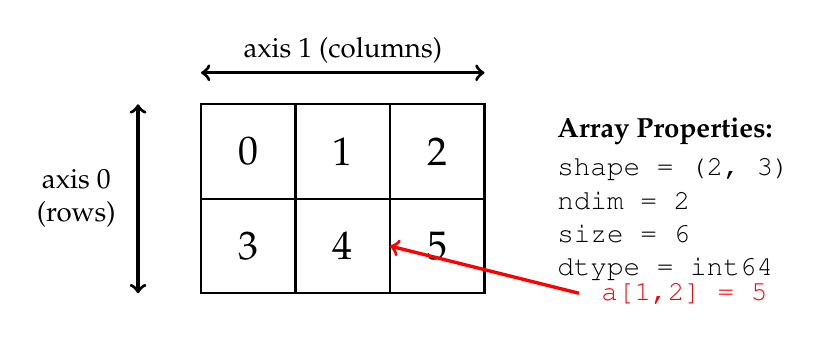
\begin{tikzpicture}[scale=0.8]
    % Draw the 2D array grid
    \foreach \i in {0,1,2} {
        \foreach \j in {0,1} {
            \pgfmathtruncatemacro{\val}{\j*3+\i}
            \draw[thick] (\i*1.5, -\j*1.5) rectangle ++(1.5, 1.5);
            \node at (\i*1.5+0.75, -\j*1.5+0.75) {\Large \val};
        }
    }
    
    % Axis labels
    \draw[<->, very thick] (-1, 1.5) -- (-1, -1.5);
    \node[left, align=center] at (-1.2, 0) {axis 0\\(rows)};
    
    \draw[<->, very thick] (0, 2.0) -- (4.5, 2.0);
    \node[above] at (2.25, 2.0) {axis 1 (columns)};
    
    % Annotations
    \node[align=left, anchor=west] at (5.5, 0) {
        \textbf{Array Properties:}\\[2pt]
        \texttt{shape = (2, 3)}\\
        \texttt{ndim = 2}\\
        \texttt{size = 6}\\
        \texttt{dtype = int64}
    };
    
    % Index example
    \draw[->, red, very thick] (6, -1.5) -- (3, -0.75);
    \node[red, right] at (6.2, -1.5) {\texttt{a[1,2] = 5}};
\end{tikzpicture}
\caption{Visual representation of a NumPy ndarray showing its multi-dimensional structure.}
\end{figure}

\section{NumPy Array Creation}

NumPy provides numerous functions for creating arrays with different initialization patterns. Mastering these creation functions is essential for efficient scientific computing.

\subsection{Converting Python Lists to NumPy Arrays}

The most straightforward way to create an array is to convert a Python list:

\begin{lstlisting}[language=Python, caption={Creating arrays from Python lists}]
import numpy as np

# 1D array from a list
a1 = np.array([1, 2, 3, 4, 5])

# 2D array from nested lists
a2 = np.array([[8, 7, 6], [5, 4, 3], [2, 1, 0]])

# 3D array from deeply nested lists
a3 = np.array([[[1, 2], [3, 4]], [[5, 6], [7, 8]]])
\end{lstlisting}

\textbf{Important note}: When creating arrays from lists, ensure that sublists have consistent lengths. Irregular nested lists will create arrays of objects rather than efficient numerical arrays.

\subsection{Creating Arrays with arange}

The \texttt{np.arange} function is similar to Python's built-in \texttt{range}, but returns a NumPy array:

\textbf{Syntax:}
\begin{lstlisting}[language=Python]
np.arange([start,] stop[, step,])
\end{lstlisting}

\textbf{Syntax Note}: The square brackets \texttt{[]} indicate optional parameters. This notation is part of EBNF (Extended Backus-Naur Form) metasyntax, a standard way to describe programming language syntax.

\textbf{Parameter breakdown:}
\begin{enumerate}
\item \texttt{start} (optional, default=0): The starting value (inclusive)
\item \texttt{stop} (required): The ending value (exclusive, not included)
\item \texttt{step} (optional, default=1): The spacing between values
\end{enumerate}

\begin{lstlisting}[language=Python, caption={Using np.arange to create arrays}]
import numpy as np

# Simple range from 0 to 9
a1 = np.arange(10)
# Result: [0, 1, 2, 3, 4, 5, 6, 7, 8, 9]

# Range with start and stop
a2 = np.arange(5, 10)
# Result: [5, 6, 7, 8, 9]

# Range with start, stop, and step
a3 = np.arange(0, 20, 2)
# Result: [0, 2, 4, 6, 8, 10, 12, 14, 16, 18]

# Can use floating-point step
a4 = np.arange(0, 1, 0.1)
# Result: [0. , 0.1, 0.2, 0.3, 0.4, 0.5, 0.6, 0.7, 0.8, 0.9]
\end{lstlisting}

\textbf{Caution with floating-point steps}: When using non-integer steps with \texttt{arange}, the exact number of elements can be unpredictable due to floating-point arithmetic imprecision. For floating-point ranges, \texttt{np.linspace} (covered next) is often preferred.

\subsection{Creating Linearly and Logarithmically Spaced Arrays}

\subsubsection{linspace: Linearly Spaced Arrays}

The \texttt{np.linspace} function creates an array of evenly spaced values over a specified range:

\textbf{Syntax:}
\begin{lstlisting}[language=Python]
np.linspace(start, stop, num)
\end{lstlisting}

\textbf{Parameter breakdown:}
\begin{enumerate}
\item \texttt{start}: The starting value (inclusive)
\item \texttt{stop}: The ending value (inclusive, unlike arange!)
\item \texttt{num}: The number of samples to generate
\end{enumerate}

\begin{lstlisting}[language=Python, caption={Using np.linspace}]
import numpy as np

# 5 evenly spaced values from 0 to 1
a1 = np.linspace(0, 1, 5)
# Result: [0.  , 0.25, 0.5 , 0.75, 1.  ]

# 10 values from -pi to pi (useful for mathematical functions)
a2 = np.linspace(-np.pi, np.pi, 10)

# 100 points from 0 to 10 (smooth for plotting)
a3 = np.linspace(0, 10, 100)
\end{lstlisting}

\textbf{Key difference from arange}: With \texttt{linspace}, you specify exactly how many points you want, and NumPy calculates the appropriate spacing. With \texttt{arange}, you specify the spacing, and NumPy calculates how many points fit.

\subsubsection{logspace: Logarithmically Spaced Arrays}

The \texttt{np.logspace} function creates an array with values that are evenly spaced on a logarithmic scale:

\textbf{Syntax:}
\begin{lstlisting}[language=Python]
np.logspace(start, stop, num)
\end{lstlisting}

\textbf{Important}: The \texttt{start} and \texttt{stop} parameters are exponents (powers of 10), not the actual values!

\begin{lstlisting}[language=Python, caption={Using np.logspace}]
import numpy as np

# 4 values from 10^0 to 10^3
a1 = np.logspace(0, 3, 4)
# Result: [1.e+00, 1.e+01, 1.e+02, 1.e+03]
# Which is: [1, 10, 100, 1000]

# 50 values from 10^-2 to 10^2 (useful for log-scale plots)
a2 = np.logspace(-2, 2, 50)
\end{lstlisting}

Logarithmic spacing is particularly useful when:
\begin{itemize}
\item Plotting data that spans several orders of magnitude
\item Analyzing systems with exponential behavior
\item Sampling frequencies for signal processing
\item Creating logarithmic axes for visualization
\end{itemize}

\subsection{Creating Uninitialized, Zero, and One Arrays}

\subsubsection{empty: Uninitialized Arrays}

The \texttt{np.empty} function creates an array without initializing its contents to any particular value:

\textbf{Syntax:}
\begin{lstlisting}[language=Python]
np.empty(shape, dtype=float)
\end{lstlisting}

\begin{lstlisting}[language=Python, caption={Creating empty arrays}]
import numpy as np

# 1D array of 5 elements
a1 = np.empty(5)

# 2D array (3 rows, 4 columns)
a2 = np.empty((3, 4))

# 3D array with specific dtype
a3 = np.empty((2, 3, 4), dtype=np.int32)
\end{lstlisting}

\textbf{Important warning}: The contents of an empty array are not predictable! They will be whatever happened to be in that memory location. Use \texttt{empty} only when you plan to immediately fill the array with computed values, as it is slightly faster than \texttt{zeros} or \texttt{ones}.

\subsubsection{zeros: Arrays Filled with Zeros}

The \texttt{np.zeros} function creates an array filled entirely with zeros:

\begin{lstlisting}[language=Python, caption={Creating arrays of zeros}]
import numpy as np

# 1D array of 5 zeros
a1 = np.zeros(5)
# Result: [0., 0., 0., 0., 0.]

# 2D array (3x4) of zeros
a2 = np.zeros((3, 4))

# Boolean array (useful for masking)
genome = np.zeros(1000, dtype=bool)
# Result: array of 1000 False values

# Integer zeros
a3 = np.zeros(10, dtype=np.int32)
\end{lstlisting}

\texttt{zeros} is commonly used for:
\begin{itemize}
\item Initializing accumulator arrays
\item Creating boolean masks (with dtype=bool)
\item Pre-allocating arrays that will be filled by computation
\end{itemize}

\subsubsection{ones: Arrays Filled with Ones}

The \texttt{np.ones} function creates an array filled with ones:

\begin{lstlisting}[language=Python, caption={Creating arrays of ones}]
import numpy as np

# 1D array of 5 ones
a1 = np.ones(5)
# Result: [1., 1., 1., 1., 1.]

# 2D array (2x3) of ones
a2 = np.ones((2, 3))

# 3D array of ones
a3 = np.ones((2, 3, 4))
\end{lstlisting}

\subsubsection{\_like Functions: Creating Arrays with Same Shape}

NumPy provides \texttt{\_like} variants that create arrays with the same shape and dtype as an existing array:

\begin{lstlisting}[language=Python, caption={Using \_like functions}]
import numpy as np

# Original array
a = np.array([[1, 2, 3], [4, 5, 6]])

# Create array of zeros with same shape as a
b = np.zeros_like(a)
# Result: [[0, 0, 0], [0, 0, 0]]

# Similarly for ones and empty
c = np.ones_like(a)
d = np.empty_like(a)
\end{lstlisting}

These functions are useful when you need to create temporary arrays for calculations that match the structure of your data.

\subsection{Creating Random Arrays}

Random number generation is fundamental to scientific computing, used in simulations, sampling, initialization, and statistical analysis.

\textbf{Modern approach (NumPy 1.17+)}: NumPy now recommends using the \texttt{default\_rng} function to create a random number generator object:

\begin{lstlisting}[language=Python, caption={Modern random number generation}]
import numpy as np

# Create a random number generator with a seed for reproducibility
rng = np.random.default_rng(42)

# Generate random floats in [0, 1)
a1 = rng.random(5)
# Result: array of 5 random floats

# 2D array of random floats
a2 = rng.random((3, 4))

# Random integers
integers = rng.integers(0, 10, size=20)
# 20 random integers from 0 to 9

# Random standard normal (Gaussian) distribution
normal = rng.standard_normal((100, 100))
\end{lstlisting}

\textbf{Why use a seed?} The seed value (42 in the example) initializes the random number generator to a known state. Using the same seed produces the same sequence of "random" numbers, which is crucial for:
\begin{itemize}
\item Debugging (you can reproduce the exact same random behavior)
\item Reproducibility of scientific results
\item Testing code
\end{itemize}

In production scientific code, you typically set a seed once at the beginning of your script, document it, and use it consistently for reproducibility.

\subsection{Complete Array Creation Example}

Here is a comprehensive example demonstrating various array creation techniques:

\begin{lstlisting}[language=Python, caption={Comprehensive array creation examples}]
import numpy as np

# From lists
a = np.array([[8, 7, 6], [5, 4, 3], [2, 1, 0]])

# Using arange (similar to range)
b = np.arange(0, 10, 2)  # [0, 2, 4, 6, 8]

# Linearly spaced
c = np.linspace(0, 1, 11)  # 11 values from 0 to 1

# Logarithmically spaced  
d = np.logspace(0, 3, 4)  # [1, 10, 100, 1000]

# Uninitialized (fast, but values unpredictable)
e = np.empty((3, 3), dtype=float)

# Zeros
f = np.zeros((5, 5))
genome = np.zeros(1000, dtype=bool)

# Ones
g = np.ones((2, 3))

# Like existing array
h = np.zeros_like(a)

# Random numbers
rng = np.random.default_rng(42)
i = rng.random((4, 4))
j = rng.standard_normal(100)

print("Array creation complete!")
\end{lstlisting}

For more array creation functions and detailed documentation, see the NumPy documentation at \url{https://numpy.org/doc/stable/reference/routines.array-creation.html}.

\section{NumPy Basic Operations}

\subsection{Element-wise Arithmetic Operations}

One of NumPy's most powerful features is that arithmetic operators work \textbf{element-wise} on arrays. This means that operations are applied to corresponding elements without the need for explicit loops.

\textbf{Critical requirement}: For element-wise operations, array shapes must be compatible! Generally, this means arrays must have the same shape, though NumPy's broadcasting rules (discussed later) provide some flexibility.

\subsubsection{Basic Arithmetic Operators}

\begin{lstlisting}[language=Python, caption={Element-wise arithmetic operations}]
import numpy as np

a = np.array([1, 2, 3, 4])
b = np.array([10, 20, 30, 40])

# Addition
c = a + b
# Result: [11, 22, 33, 44]

# Subtraction
d = a - b
# Result: [-9, -18, -27, -36]

# Multiplication (element-wise, not matrix multiplication!)
e = a * b
# Result: [10, 40, 90, 160]

# Division
f = b / a
# Result: [10., 20., 30., 40.]

# Exponentiation
g = a**b
# Result: [1, 1048576, ..., ...] (extremely large numbers!)

# Integer division
h = b // a
# Result: [10, 10, 10, 10]

# Modulo
i = b % a
# Result: [0, 0, 0, 0]
\end{lstlisting}

\textbf{Important distinction}: The \texttt{*} operator performs element-wise multiplication, NOT matrix multiplication. For matrix multiplication, use the \texttt{@} operator or \texttt{np.dot()}.

\subsubsection{Multi-dimensional Operations}

Element-wise operations work seamlessly with multi-dimensional arrays:

\begin{lstlisting}[language=Python, caption={Operations on multi-dimensional arrays}]
import numpy as np

# 2D arrays
A = np.array([[1, 2], [3, 4]])
B = np.array([[5, 6], [7, 8]])

# Element-wise operations work identically
C = A + B
# Result: [[ 6,  8],
#          [10, 12]]

D = A * B  # Element-wise multiplication
# Result: [[ 5, 12],
#          [21, 32]]

E = A @ B  # Matrix multiplication
# Result: [[19, 22],
#          [43, 50]]
\end{lstlisting}

\subsection{Universal Functions (ufuncs)}

NumPy provides a large collection of mathematical functions that operate element-wise on arrays. These are called \textbf{universal functions} or \textbf{ufuncs}.

\subsubsection{Trigonometric Functions}

\begin{lstlisting}[language=Python, caption={Trigonometric ufuncs}]
import numpy as np

# Create an array of angles
theta = np.linspace(0, 2*np.pi, 100)

# Apply trigonometric functions
sin_values = np.sin(theta)
cos_values = np.cos(theta)
tan_values = np.tan(theta)

# These work element-wise on entire arrays!
# No loops needed!
\end{lstlisting}

\subsubsection{Mathematical Functions}

\begin{lstlisting}[language=Python, caption={Mathematical ufuncs}]
import numpy as np

a = np.array([1, 4, 9, 16, 25])

# Square root
b = np.sqrt(a)
# Result: [1., 2., 3., 4., 5.]

# Exponential
c = np.exp(a)
# Result: [2.71828..., 54.598..., ...]

# Natural logarithm
d = np.log(a)
# Result: [0., 1.386..., 2.197..., ...]

# Absolute value
e = np.array([-5, -3, 0, 3, 5])
f = np.abs(e)
# Result: [5, 3, 0, 3, 5]
\end{lstlisting}

\subsubsection{Aggregation Functions}

Aggregation functions reduce an array to a single value (or along specified axes):

\begin{lstlisting}[language=Python, caption={Aggregation functions}]
import numpy as np

a = np.array([1, 2, 3, 4, 5])

# Sum of all elements
total = np.sum(a)
# Result: 15

# Minimum and maximum
minimum = np.min(a)
# Result: 1
maximum = np.max(a)
# Result: 5

# Mean (average)
average = np.mean(a)
# Result: 3.0

# Standard deviation
std_dev = np.std(a)
# Result: 1.414...

# Median
median = np.median(a)
# Result: 3.0
\end{lstlisting}

\textbf{Aggregating along axes in multi-dimensional arrays}:

\begin{lstlisting}[language=Python, caption={Axis-wise aggregations}]
import numpy as np

# 2D array
A = np.array([[1, 2, 3],
              [4, 5, 6],
              [7, 8, 9]])

# Sum all elements
total = np.sum(A)
# Result: 45

# Sum along axis 0 (down columns)
col_sums = np.sum(A, axis=0)
# Result: [12, 15, 18]

# Sum along axis 1 (across rows)
row_sums = np.sum(A, axis=1)
# Result: [ 6, 15, 24]

# Mean of each column
col_means = np.mean(A, axis=0)
# Result: [4., 5., 6.]
\end{lstlisting}

\textbf{Understanding axes}: For a 2D array:
\begin{itemize}
\item \texttt{axis=0} operates down the rows (across different rows, within each column)
\item \texttt{axis=1} operates across the columns (across different columns, within each row)
\end{itemize}

Mnemonic: The axis you specify is the one that "disappears" in the result.

\subsection{Complete Operations Example}

\begin{lstlisting}[language=Python, caption={Comprehensive example of NumPy operations}]
import numpy as np

# Create arrays
a = np.array([1, 2, 3, 4, 5])
b = np.array([5, 4, 3, 2, 1])

# Basic arithmetic (element-wise)
sum_ab = a + b        # [6, 6, 6, 6, 6]
diff_ab = a - b       # [-4, -2, 0, 2, 4]
prod_ab = a * b       # [5, 8, 9, 8, 5]
quot_ab = a / b       # [0.2, 0.5, 1. , 2. , 5. ]
power_ab = a**2       # [1, 4, 9, 16, 25]

# Universal functions
sqrt_a = np.sqrt(a)   # [1., 1.414..., 1.732..., 2., 2.236...]
sin_a = np.sin(a)     # [0.841..., 0.909..., 0.141..., ...]
exp_a = np.exp(a)     # [2.718..., 7.389..., 20.085..., ...]

# Aggregations
total = np.sum(a)     # 15
mean = np.mean(a)     # 3.0
std = np.std(a)       # 1.414...
minimum = np.min(a)   # 1
maximum = np.max(a)   # 5

print("Operations completed successfully!")
\end{lstlisting}

\textbf{Performance note}: All of these operations are vectorized, meaning they execute in highly optimized compiled code without Python loops. This is what makes NumPy dramatically faster than pure Python for numerical computations.

For a complete list of NumPy's mathematical functions, see: \url{https://numpy.org/doc/stable/reference/routines.math.html}

\section{NumPy Indexing and Slicing}

Indexing and slicing are fundamental operations for accessing and manipulating array data. NumPy extends Python's list indexing to multiple dimensions, providing powerful and flexible data access.

\subsection{One-Dimensional Indexing and Slicing}

NumPy's 1D indexing is similar to Python list indexing, but with additional capabilities:

\subsubsection{Basic Slicing Syntax}

\textbf{Syntax:}
\begin{lstlisting}[language=Python]
array[start:end:step]
\end{lstlisting}

\textbf{Component breakdown:}
\begin{enumerate}
\item \texttt{start}: Index where slice begins (inclusive), default is 0
\item \texttt{end}: Index where slice ends (exclusive), default is len(array)
\item \texttt{step}: Increment between indices, default is 1
\end{enumerate}

\begin{lstlisting}[language=Python, caption={One-dimensional slicing}]
import numpy as np

a = np.array([0, 1, 2, 3, 4, 5, 6, 7, 8, 9])

# Elements from index 1 to 3 (exclusive)
b = a[1:4]
# Result: [1, 2, 3]

# From index 1 to end
c = a[1:]
# Result: [1, 2, 3, 4, 5, 6, 7, 8, 9]

# From beginning until index 7 (exclusive)
d = a[0:-1]
# Result: [0, 1, 2, 3, 4, 5, 6, 7, 8]
# Note: -1 means "last element"

# With step size
e = a[0:7:2]
# Result: [0, 2, 4, 6]
# Every 2nd element from 0 to 6

# Reverse with negative step
f = a[-1:0:-2]
# Result: [9, 7, 5, 3, 1]
# Start from last, go backwards by 2

# Reverse entire array
g = a[::-1]
# Result: [9, 8, 7, 6, 5, 4, 3, 2, 1, 0]

# Every other element in reverse
h = a[::-2]
# Result: [9, 7, 5, 3, 1]
\end{lstlisting}

\textbf{Understanding negative indices}:
\begin{itemize}
\item \texttt{-1} refers to the last element
\item \texttt{-2} refers to the second-to-last element
\item And so on
\end{itemize}

This is particularly useful for accessing elements from the end without knowing the array's length.

\subsection{Multi-dimensional Indexing and Slicing}

For multi-dimensional arrays, NumPy extends slicing to each dimension using comma-separated indices or slices.

\textbf{Syntax for multi-dimensional slicing}:
\begin{lstlisting}[language=Python]
array[slice_dim0, slice_dim1, slice_dim2, ...]
\end{lstlisting}

Each dimension is specified separately, separated by commas, forming a tuple of indices.

\subsubsection{2D Array Examples}

\begin{lstlisting}[language=Python, caption={Two-dimensional slicing}]
import numpy as np

# Create a 5x6 array
a = np.arange(30).reshape(5, 6)
# Result:
# [[ 0,  1,  2,  3,  4,  5],
#  [ 6,  7,  8,  9, 10, 11],
#  [12, 13, 14, 15, 16, 17],
#  [18, 19, 20, 21, 22, 23],
#  [24, 25, 26, 27, 28, 29]]

# Single element: row 2, column 3
element = a[2, 3]
# Result: 15

# Entire row (row 2)
row = a[2, :]
# Result: [12, 13, 14, 15, 16, 17]

# Entire column (column 3)
column = a[:, 3]
# Result: [ 3,  9, 15, 21, 27]

# Subarray (rows 1-3, columns 2-4)
subarray = a[1:3, 2:5]
# Result:
# [[ 8,  9, 10],
#  [14, 15, 16]]

# Every other row, all columns
every_other_row = a[::2, :]
# Result:
# [[ 0,  1,  2,  3,  4,  5],
#  [12, 13, 14, 15, 16, 17],
#  [24, 25, 26, 27, 28, 29]]
\end{lstlisting}

\subsubsection{3D Array Examples}

\begin{lstlisting}[language=Python, caption={Three-dimensional slicing}]
import numpy as np

# Create a 3D array (shape: 3, 4, 5)
a = np.arange(60).reshape(3, 4, 5)

# All elements in last dimension, 
# at specific position in first two dimensions
slice1 = a[1, 2, :]
# Extracts a 1D array

# All elements along axis 0 and 1, 
# specific position along axis 2
slice2 = a[:, :, 3]
# Extracts a 2D array (all "layers" at position 3)

# First two "layers", middle rows
slice3 = a[0:2, 1:3, :]
# Extracts a 3D subarray with shape (2, 2, 5)
\end{lstlisting}

\subsection{Important Concepts: Views vs Copies}

\textbf{Critical concept}: When you slice a NumPy array, you typically get a \textbf{view}, not a copy. This means the sliced array shares memory with the original array. Modifying the slice modifies the original!

\begin{lstlisting}[language=Python, caption={Views vs Copies demonstration}]
import numpy as np

a = np.array([0, 1, 2, 3, 4, 5])

# Create a slice (this is a view!)
b = a[2:5]
# b is [2, 3, 4]

# Modify the slice
b[0] = 999

# Check original array - it's also modified!
print(a)
# Result: [0, 1, 999, 3, 4, 5]

# To create an independent copy
c = a[2:5].copy()
c[0] = -1
print(a)  # Original unchanged
\end{lstlisting}

This behavior is intentional and provides significant performance benefits (no unnecessary copying of large arrays), but you must be aware of it to avoid unexpected modifications.

\subsection{Advanced Indexing Techniques}

\subsubsection{Boolean Indexing}

You can use boolean arrays to select elements:

\begin{lstlisting}[language=Python, caption={Boolean indexing}]
import numpy as np

a = np.array([10, 15, 20, 25, 30])

# Create boolean mask
mask = a > 18
# Result: [False, False, True, True, True]

# Use mask to select elements
selected = a[mask]
# Result: [20, 25, 30]

# Can do this in one line
selected2 = a[a > 18]
# Same result
\end{lstlisting}

\subsubsection{Integer Array Indexing}

You can use arrays of indices to select specific elements:

\begin{lstlisting}[language=Python, caption={Integer array indexing}]
import numpy as np

a = np.array([10, 20, 30, 40, 50])

# Select specific indices
indices = np.array([0, 2, 4])
selected = a[indices]
# Result: [10, 30, 50]

# Works for multi-dimensional too
A = np.arange(20).reshape(4, 5)
rows = np.array([0, 2, 3])
cols = np.array([1, 3, 4])
selected_elements = A[rows, cols]
# Result: [1, 13, 19]
\end{lstlisting}

% \begin{figure}[h!]
% \centering
% \includegraphics[width=0.8\textwidth]{placeholder_numpy_slicing_diagram.png}
% \caption{Visual representation of NumPy array slicing in 2D, showing how different slicing operations select subarrays. The diagram illustrates row slicing, column slicing, and rectangular subarray extraction with corresponding index notation.}
% \label{fig:numpy_slicing}
% \end{figure}

\begin{figure}[h!]
\centering
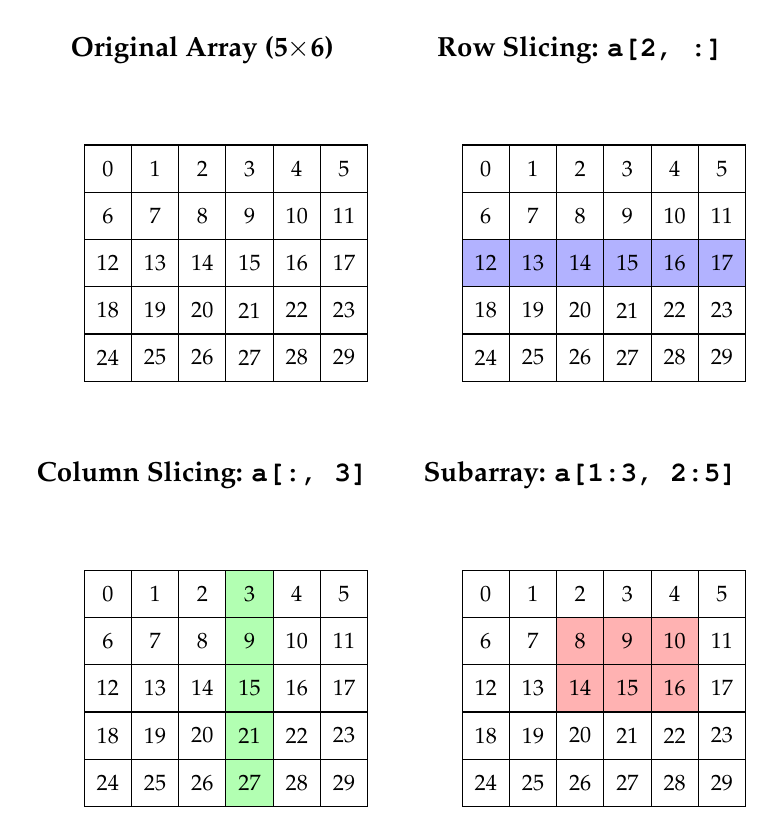
\begin{tikzpicture}[scale=0.6]
    % Original array
    \node at (2.5, 3) {\textbf{Original Array (5$\times$6)}};
    \foreach \i in {0,...,4} {
        \foreach \j in {0,...,5} {
            \pgfmathtruncatemacro{\val}{\i*6+\j}
            \draw ({\j}, {-\i}) rectangle ++(1, 1);
            \node at ({\j+0.5}, {-\i+0.5}) {\footnotesize \val};
        }
    }
    
    % Row slicing example
    \begin{scope}[xshift=8cm]
        \node at (2.5, 3) {\textbf{Row Slicing: \texttt{a[2, :]}}};
        \foreach \i in {0,...,4} {
            \foreach \j in {0,...,5} {
                \pgfmathtruncatemacro{\val}{\i*6+\j}
                \ifnum\i=2
                    \fill[blue!30] ({\j}, {-\i}) rectangle ++(1, 1);
                \fi
                \draw ({\j}, {-\i}) rectangle ++(1, 1);
                \node at ({\j+0.5}, {-\i+0.5}) {\footnotesize \val};
            }
        }
    \end{scope}
    
    % Column slicing example
    \begin{scope}[yshift=-9cm]
        \node at (2.5, 3) {\textbf{Column Slicing: \texttt{a[:, 3]}}};
        \foreach \i in {0,...,4} {
            \foreach \j in {0,...,5} {
                \pgfmathtruncatemacro{\val}{\i*6+\j}
                \ifnum\j=3
                    \fill[green!30] ({\j}, {-\i}) rectangle ++(1, 1);
                \fi
                \draw ({\j}, {-\i}) rectangle ++(1, 1);
                \node at ({\j+0.5}, {-\i+0.5}) {\footnotesize \val};
            }
        }
    \end{scope}
    
    % Subarray slicing
    \begin{scope}[xshift=8cm, yshift=-9cm]
        \node at (2.5, 3) {\textbf{Subarray: \texttt{a[1:3, 2:5]}}};
        \foreach \i in {0,...,4} {
            \foreach \j in {0,...,5} {
                \pgfmathtruncatemacro{\val}{\i*6+\j}
                \ifnum\i>0
                    \ifnum\i<3
                        \ifnum\j>1
                            \ifnum\j<5
                                \fill[red!30] ({\j}, {-\i}) rectangle ++(1, 1);
                            \fi
                        \fi
                    \fi
                \fi
                \draw ({\j}, {-\i}) rectangle ++(1, 1);
                \node at ({\j+0.5}, {-\i+0.5}) {\footnotesize \val};
            }
        }
    \end{scope}
\end{tikzpicture}
\caption{Visual representation of NumPy array slicing in 2D.}
\end{figure}

\section{Broadcasting: Operating on Arrays of Different Shapes}

\subsection{Introduction to Broadcasting}

\textbf{Broadcasting} is a powerful mechanism that allows NumPy to perform operations on arrays of different shapes. Under certain conditions, the smaller array is "broadcast" across the larger array so that they have compatible shapes.

\textbf{Why is broadcasting important?} Broadcasting eliminates the need for explicit loops or array replication, making code more concise, readable, and efficient. It's one of NumPy's most elegant features.

\subsection{Simple Broadcasting Example}

The simplest case of broadcasting is operating between an array and a scalar:

\begin{lstlisting}[language=Python, caption={Broadcasting with scalars}]
import numpy as np

a = np.array([1, 2, 3, 4])

# Add scalar to array
b = a + 10
# Result: [11, 12, 13, 14]
# The scalar 10 is "broadcast" to [10, 10, 10, 10]

# Multiply array by scalar
c = a * 2
# Result: [2, 4, 6, 8]
\end{lstlisting}

\subsection{Broadcasting Rules}

NumPy compares array shapes element-wise starting from the trailing dimensions. Two dimensions are compatible when:

\begin{enumerate}
\item They are equal, OR
\item One of them is 1
\end{enumerate}

If these conditions are not met, a \texttt{ValueError} is raised.

\textbf{Examples of compatible shapes}:
\begin{itemize}
\item \texttt{(3, 4)} and \texttt{(4,)} → compatible, result shape \texttt{(3, 4)}
\item \texttt{(5, 1)} and \texttt{(1, 4)} → compatible, result shape \texttt{(5, 4)}
\item \texttt{(3, 4, 5)} and \texttt{(5,)} → compatible, result shape \texttt{(3, 4, 5)}
\item \texttt{(3, 4, 5)} and \texttt{(4, 5)} → compatible, result shape \texttt{(3, 4, 5)}
\end{itemize}

\textbf{Examples of incompatible shapes}:
\begin{itemize}
\item \texttt{(3, 4)} and \texttt{(5,)} → incompatible (trailing dimensions 4 and 5 don't match)
\item \texttt{(3, 4)} and \texttt{(3,)} → incompatible (would need to match trailing dimensions)
\end{itemize}

\subsection{Broadcasting Examples}

\begin{lstlisting}[language=Python, caption={Various broadcasting scenarios}]
import numpy as np

# 1D array broadcast to 2D
a = np.array([[1, 2, 3],
              [4, 5, 6],
              [7, 8, 9]])  # Shape: (3, 3)

b = np.array([10, 20, 30])  # Shape: (3,)

c = a + b
# b is broadcast to shape (3, 3):
# [[10, 20, 30],
#  [10, 20, 30],
#  [10, 20, 30]]
# Result:
# [[11, 22, 33],
#  [14, 25, 36],
#  [17, 28, 39]]

# Column vector broadcast
d = np.array([[10],
              [20],
              [30]])  # Shape: (3, 1)

e = a + d
# d is broadcast to shape (3, 3):
# [[10, 10, 10],
#  [20, 20, 20],
#  [30, 30, 30]]
# Result:
# [[11, 12, 13],
#  [24, 25, 26],
#  [37, 38, 39]]
\end{lstlisting}

\subsection{Broadcasting Documentation}

Broadcasting is a sophisticated topic with many nuances. For the complete, authoritative explanation with visual diagrams, see NumPy's official documentation: \url{https://numpy.org/doc/stable/user/basics.broadcasting.html}

This documentation includes:
\begin{itemize}
\item Detailed rules for broadcasting
\item Visual diagrams showing how arrays are broadcast
\item Examples of common broadcasting patterns
\item Performance implications
\end{itemize}

% \begin{figure}[h!]
% \centering
% \includegraphics[width=0.7\textwidth]{placeholder_broadcasting_visualization.png}
% \caption{Visual representation of NumPy broadcasting, showing how a 1D array is broadcast to match a 2D array's shape. The diagram illustrates the conceptual expansion of the smaller array without actual data duplication.}
% \label{fig:broadcasting}
% \end{figure}

\begin{figure}[h!]
\centering
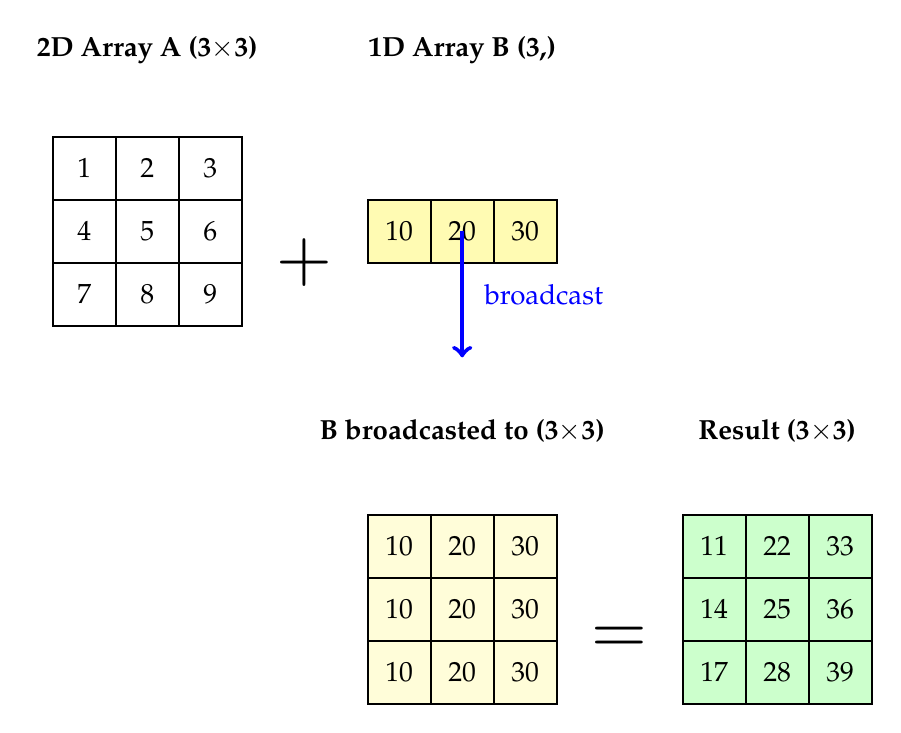
\begin{tikzpicture}[scale=0.8]
    % 2D Array A (3x3)
    \node[above] at (1.5, 2) {\textbf{2D Array A (3$\times$3)}};
    \foreach \i in {0,1,2} {
        \foreach \j in {0,1,2} {
            \pgfmathtruncatemacro{\val}{\i*3+\j+1}
            \draw[thick] (\j, -\i) rectangle ++(1, 1);
            \node at (\j+0.5, -\i+0.5) {\val};
        }
    }
    
    % Plus sign
    \node at (4, -1) {\Huge $+$};
    
    % 1D Array B (3,)
    \node[above] at (6.5, 2) {\textbf{1D Array B (3,)}};
    \foreach \j in {0,1,2} {
        \pgfmathtruncatemacro{\val}{(\j+1)*10}
        \draw[thick, fill=yellow!30] (5+\j, -1) rectangle ++(1, 1);
        \node at (5.5+\j, -0.5) {\val};
    }
    
    % Arrow indicating broadcast
    \draw[->, ultra thick, blue] (6.5, -0.5) -- (6.5, -2.5);
    \node[right, blue] at (6.7, -1.5) {broadcast};
    
    % Broadcasted version
    \begin{scope}[yshift=-6cm]
        \node[above] at (6.5, 2) {\textbf{B broadcasted to (3$\times$3)}};
        \foreach \i in {0,1,2} {
            \foreach \j in {0,1,2} {
                \pgfmathtruncatemacro{\val}{(\j+1)*10}
                \draw[thick, fill=yellow!15] (5+\j, -\i) rectangle ++(1, 1);
                \node at (5.5+\j, -\i+0.5) {\val};
            }
        }
    \end{scope}
    
    % Equals sign
    \node at (9, -7) {\Huge $=$};
    
    % Result
    \begin{scope}[xshift=10cm, yshift=-6cm]
        \node[above] at (1.5, 2) {\textbf{Result (3$\times$3)}};
        \foreach \i in {0,1,2} {
            \foreach \j in {0,1,2} {
                \pgfmathtruncatemacro{\vala}{\i*3+\j+1}
                \pgfmathtruncatemacro{\valb}{(\j+1)*10}
                \pgfmathtruncatemacro{\result}{\vala+\valb}
                \draw[thick, fill=green!20] (\j, -\i) rectangle ++(1, 1);
                \node at (\j+0.5, -\i+0.5) {\result};
            }
        }
    \end{scope}
\end{tikzpicture}
\caption{Visual representation of NumPy broadcasting.}
\end{figure}

\section{Practical Example: Solving the Poisson Equation}

\subsection{Introduction to the Poisson Equation}

To demonstrate the power of NumPy in scientific computing, we now explore a complete, practical example: numerically solving the \textbf{Poisson equation}. This example illustrates how NumPy's array operations translate directly to mathematical expressions, enabling elegant and efficient implementations of numerical algorithms.

\subsection{Mathematical Background}

The Poisson equation is a fundamental partial differential equation (PDE) that appears throughout physics and engineering:

\[
\nabla^2 u = f
\]

Or in 2D Cartesian coordinates:

\[
\frac{\partial^2 u}{\partial x^2} + \frac{\partial^2 u}{\partial y^2} = f(x, y)
\]

with boundary conditions specified on the domain boundary:

\[
u|_{\partial \Omega} = g
\]

where:
\begin{itemize}
\item $u(x, y)$ is the unknown function we want to find
\item $f(x, y)$ is a known source term
\item $\Omega$ is the domain (region where we solve the equation)
\item $\partial \Omega$ is the boundary of the domain
\item $g$ specifies the values on the boundary
\end{itemize}

\textbf{Physical applications}: This equation models numerous physical phenomena:
\begin{itemize}
\item \textbf{Heat conduction}: $u$ represents temperature, $f$ represents heat sources
\item \textbf{Electromagnetism}: $u$ represents electric or magnetic potential
\item \textbf{Astrophysics}: $u$ represents gravitational potential
\item \textbf{Fluid dynamics}: appears in pressure-velocity formulations
\end{itemize}

The Poisson equation is the simplest example of an \textbf{elliptic partial differential equation}, making it an ideal starting point for learning numerical PDE methods.

\subsection{Discretization: From Continuous to Discrete}

Since computers work with discrete values, we must discretize the continuous domain and differential operators.

\subsubsection{Domain Discretization}

Consider a square domain $\Omega = [0, L] \times [0, L]$. We divide it into a regular grid with spacing $\Delta x$ and $\Delta y$:

\begin{itemize}
\item Number of points in $x$-direction: $n_x$
\item Number of points in $y$-direction: $n_y$
\item Grid spacing: $\Delta x = L / (n_x - 1)$, $\Delta y = L / (n_y - 1)$
\item Grid points: $(x_i, y_j)$ where $x_i = i \cdot \Delta x$, $y_j = j \cdot \Delta y$
\end{itemize}

We represent the continuous function $u(x, y)$ by its values at grid points: $u_{i,j} = u(x_i, y_j)$.

% \begin{figure}[h!]
% \centering
% \includegraphics[width=0.5\textwidth]{placeholder_domain_discretization.png}
% \caption{Discretization of a square domain showing grid points and spacing. The domain is divided into a regular grid with spacing $\Delta x$ and $\Delta y$, with boundary points clearly marked.}
% \label{fig:domain_discretization}
% \end{figure}

\begin{figure}[h!]
\centering
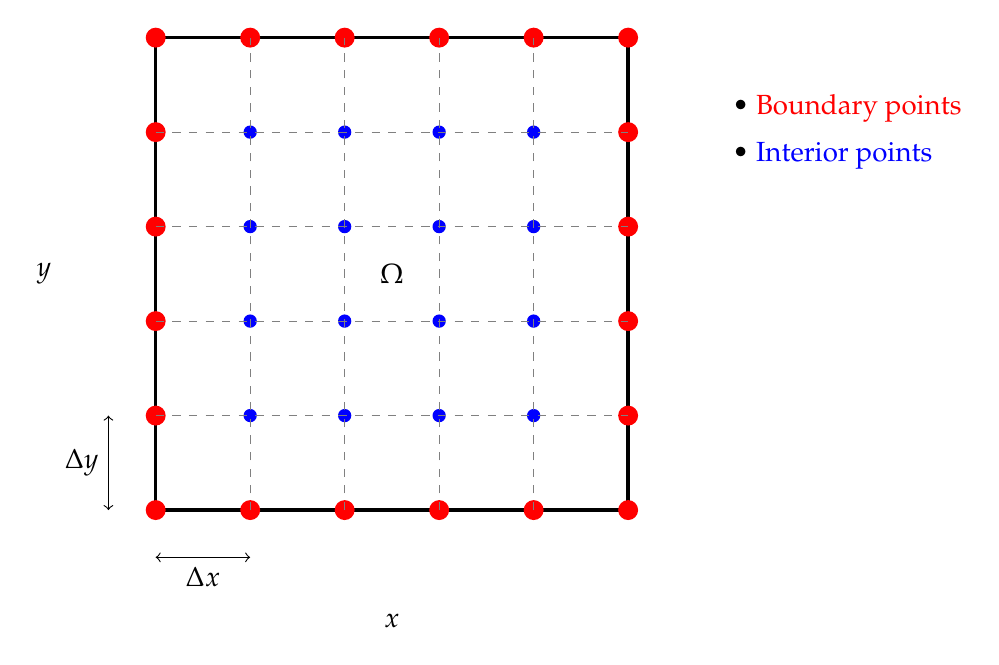
\begin{tikzpicture}[scale=1.2]
    % Draw domain boundary
    \draw[very thick] (0,0) rectangle (5,5);
    
    % Draw grid points
    \foreach \i in {0,...,5} {
        \foreach \j in {0,...,5} {
            \ifnum\i=0
                \fill[red] (\i, \j) circle (3pt);
            \else\ifnum\i=5
                \fill[red] (\i, \j) circle (3pt);
            \else\ifnum\j=0
                \fill[red] (\i, \j) circle (3pt);
            \else\ifnum\j=5
                \fill[red] (\i, \j) circle (3pt);
            \else
                \fill[blue] (\i, \j) circle (2pt);
            \fi\fi\fi\fi
        }
    }
    
    % Draw grid lines (dashed)
    \foreach \i in {1,...,4} {
        \draw[gray, dashed] (\i, 0) -- (\i, 5);
        \draw[gray, dashed] (0, \i) -- (5, \i);
    }
    
    % Spacing annotations
    \draw[<->] (0, -0.5) -- (1, -0.5);
    \node[below] at (0.5, -0.5) {$\Delta x$};
    
    \draw[<->] (-0.5, 0) -- (-0.5, 1);
    \node[left] at (-0.5, 0.5) {$\Delta y$};
    
    % Axis labels
    \node[below] at (2.5, -1) {$x$};
    \node[left] at (-1, 2.5) {$y$};
    
    % Legend
    \node[anchor=west, align=left] at (6, 4) {
        \textbullet\ {\color{red} Boundary points}\\[5pt]
        \textbullet\ {\color{blue} Interior points}
    };
    
    % Domain label
    \node at (2.5, 2.5) {$\Omega$};
\end{tikzpicture}
\caption{Discretization of a square domain showing grid points and spacing.}
\end{figure}

\subsubsection{Finite Difference Approximation}

The second derivatives in the Poisson equation are approximated using \textbf{finite differences}. The standard centered difference formula gives:

\[
\frac{\partial^2 u}{\partial x^2}\bigg|_{i,j} \approx \frac{u_{i+1,j} - 2u_{i,j} + u_{i-1,j}}{(\Delta x)^2}
\]

\[
\frac{\partial^2 u}{\partial y^2}\bigg|_{i,j} \approx \frac{u_{i,j+1} - 2u_{i,j} + u_{i,j-1}}{(\Delta y)^2}
\]

The Poisson equation at grid point $(i,j)$ becomes:

\[
\frac{u_{i+1,j} - 2u_{i,j} + u_{i-1,j}}{(\Delta x)^2} + \frac{u_{i,j+1} - 2u_{i,j} + u_{i,j-1}}{(\Delta y)^2} = f_{i,j}
\]

% \begin{figure}[h!]
% \centering
% \includegraphics[width=0.6\textwidth]{placeholder_finite_difference_stencil.png}
% \caption{The five-point finite difference stencil for the 2D Laplacian operator. The diagram shows how the value at point $(i,j)$ depends on its four neighbors, illustrating the discretization pattern used in the numerical solution.}
% \label{fig:fd_stencil}
% \end{figure}

\begin{figure}[h!]
\centering
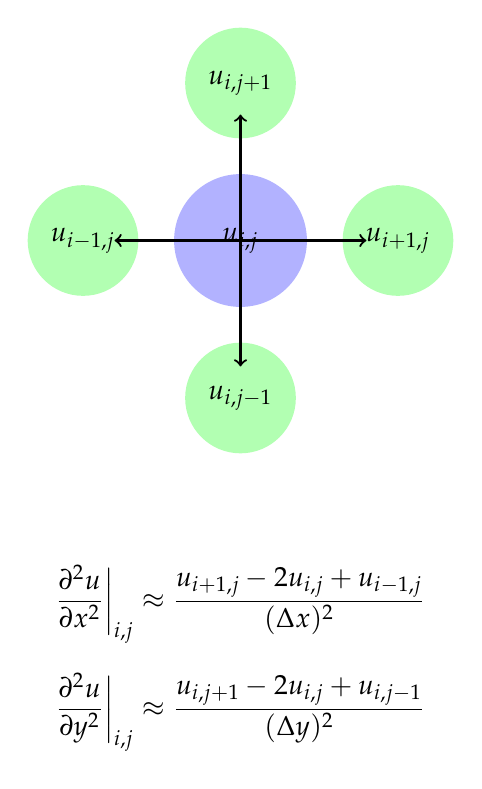
\begin{tikzpicture}[scale=2]
    % Draw grid points
    \fill[blue!30] (0,0) circle (12pt);
    \node at (0,0) {$u_{i,j}$};
    
    \fill[green!30] (1,0) circle (10pt);
    \node at (1,0) {$u_{i+1,j}$};
    
    \fill[green!30] (-1,0) circle (10pt);
    \node at (-1,0) {$u_{i-1,j}$};
    
    \fill[green!30] (0,1) circle (10pt);
    \node at (0,1) {$u_{i,j+1}$};
    
    \fill[green!30] (0,-1) circle (10pt);
    \node at (0,-1) {$u_{i,j-1}$};
    
    % Draw connecting lines
    \draw[->, thick] (0,0) -- (0.8,0);
    \draw[->, thick] (0,0) -- (-0.8,0);
    \draw[->, thick] (0,0) -- (0,0.8);
    \draw[->, thick] (0,0) -- (0,-0.8);
    
    % Formula below
    \node[align=center, below] at (0, -2) {
        $\displaystyle \frac{\partial^2 u}{\partial x^2}\bigg|_{i,j} \approx \frac{u_{i+1,j} - 2u_{i,j} + u_{i-1,j}}{(\Delta x)^2}$\\[10pt]
        $\displaystyle \frac{\partial^2 u}{\partial y^2}\bigg|_{i,j} \approx \frac{u_{i,j+1} - 2u_{i,j} + u_{i,j-1}}{(\Delta y)^2}$
    };
\end{tikzpicture}
\caption{The five-point finite difference stencil for the 2D Laplacian operator.}
\end{figure}

\subsection{The Jacobi Iterative Method}

To solve the resulting system of equations, we use the \textbf{Jacobi iterative method}. This method starts with an initial guess and iteratively improves the solution.

\textbf{Algorithm}: Given current values $u^{(k)}$, compute new values $u^{(k+1)}$:

For $\Delta x = \Delta y$ (square grid):

\[
u^{(k+1)}_{i,j} = \frac{1}{4}\left(u^{(k)}_{i+1,j} + u^{(k)}_{i-1,j} + u^{(k)}_{i,j+1} + u^{(k)}_{i,j-1} - (\Delta x)^2 f_{i,j}\right)
\]

For general $\Delta x$, $\Delta y$:

\[
u^{(k+1)}_{i,j} = \frac{(u^{(k)}_{i+1,j} + u^{(k)}_{i-1,j})(\Delta y)^2 + (u^{(k)}_{i,j+1} + u^{(k)}_{i,j-1})(\Delta x)^2 - f_{i,j}(\Delta x)^2(\Delta y)^2}{2((\Delta x)^2 + (\Delta y)^2)}
\]

This process is repeated until the solution converges (stops changing significantly).

\begin{figure}[h!]
\centering
\includegraphics[width=1\textwidth]{placeholder_jacobi_convergence.png}
\caption{Visual representation of the Jacobi iteration process showing convergence over multiple iterations. The sequence of plots illustrates how the initial guess gradually approaches the true solution.}
\label{fig:jacobi_convergence}
\end{figure}

\subsection{Implementation Comparison: Loops vs Vectorization}

Now we compare two implementations of the Jacobi iteration: one using explicit Python loops, and one using NumPy's vectorized operations.

\subsubsection{Loop-based Implementation}

\begin{lstlisting}[language=Python, caption={Loop-based Jacobi update (slow)}]
def update(u, f, dx, dy):
    """Update solution using explicit loops"""
    [nx, ny] = u.shape
    dx2 = dx**2
    dy2 = dy**2
    
    # Create a copy of current values
    u_old = np.copy(u)
    
    # Loop over interior points
    for i in range(1, nx-1):
        for j in range(1, ny-1):
            u[i,j] = ((u_old[i+1,j ] + u_old[i-1,j ])*dy2 +
                      (u_old[i ,j+1] + u_old[i ,j-1])*dx2 -
                      f[i,j]*dx2*dy2) / (2*(dx2 + dy2))
\end{lstlisting}

\textbf{Analysis of loop-based approach}:
\begin{itemize}
\item Two nested loops iterate over interior grid points
\item Each grid point update involves Python interpreter overhead
\item Relatively slow for large grids
\item Clear correspondence to mathematical formula
\item Easy to understand for beginners
\end{itemize}

\subsubsection{Vectorized Implementation}

\begin{lstlisting}[language=Python, caption={Vectorized Jacobi update (fast)}]
def update(u, f, dx, dy):
    """Update solution using NumPy array slicing"""
    dx2 = dx**2
    dy2 = dy**2
    
    # Create a copy of current values
    u_old = np.copy(u)
    
    # Vectorized update for all interior points at once!
    u[1:-1,1:-1] = ((u_old[2:,1:-1] + u_old[:-2,1:-1])*dy2 +
                     (u_old[1:-1,2:] + u_old[1:-1,:-2])*dx2 -
                     f[1:-1,1:-1]*dx2*dy2) / (2*(dx2 + dy2))
\end{lstlisting}

\textbf{Analysis of vectorized approach}:
\begin{itemize}
\item \textbf{No explicit loops!} All operations are array operations
\item \texttt{u[1:-1,1:-1]} selects all interior points
\item \texttt{u[2:,1:-1]} selects right neighbors (i+1, j)
\item \texttt{u[:-2,1:-1]} selects left neighbors (i-1, j)
\item \texttt{u[1:-1,2:]} selects upper neighbors (i, j+1)
\item \texttt{u[1:-1,:-2]} selects lower neighbors (i, j-1)
\item Dramatically faster (often 50-100x speedup)
\item Operations execute in optimized C code
\end{itemize}

\subsubsection{Understanding the Slicing}

The vectorized version uses clever slicing to select neighbor points:

\begin{lstlisting}[language=Python, caption={Breaking down the slicing operations}]
# For an array of shape (nx, ny):

# Interior points: all points except boundaries
interior = u[1:-1, 1:-1]         # Shape: (nx-2, ny-2)

# Right neighbors (i+1, j):
right = u[2:, 1:-1]              # Starts from row 2, goes to end
                                  # Same as u[i+1, j] for each i

# Left neighbors (i-1, j):
left = u[:-2, 1:-1]              # Starts from row 0, ends at -2
                                  # Same as u[i-1, j] for each i

# Upper neighbors (i, j+1):
upper = u[1:-1, 2:]              # Same rows, starts from column 2

# Lower neighbors (i, j-1):
lower = u[1:-1, :-2]             # Same rows, ends at column -2
\end{lstlisting}

All these slices have the same shape \texttt{(nx-2, ny-2)}, so they can be combined in a single vectorized expression!

\subsection{Complete Working Example}

\begin{lstlisting}[language=Python, caption={Complete Poisson solver with Jacobi iteration}]
import numpy as np
import matplotlib.pyplot as plt

def solve_poisson_2d(nx, ny, dx, dy, f, u_boundary, max_iter=1000, tol=1e-6):
    """
    Solve 2D Poisson equation using Jacobi iteration
    
    Parameters:
    -----------
    nx, ny : int
        Number of grid points in x and y directions
    dx, dy : float
        Grid spacing in x and y directions
    f : ndarray
        Source term array (nx, ny)
    u_boundary : ndarray
        Boundary values (nx, ny)
    max_iter : int
        Maximum number of iterations
    tol : float
        Convergence tolerance
        
    Returns:
    --------
    u : ndarray
        Solution array
    iterations : int
        Number of iterations performed
    """
    # Initialize solution with boundary values
    u = u_boundary.copy()
    dx2 = dx**2
    dy2 = dy**2
    
    for iteration in range(max_iter):
        u_old = u.copy()
        
        # Vectorized Jacobi update
        u[1:-1,1:-1] = ((u_old[2:,1:-1] + u_old[:-2,1:-1])*dy2 +
                         (u_old[1:-1,2:] + u_old[1:-1,:-2])*dx2 -
                         f[1:-1,1:-1]*dx2*dy2) / (2*(dx2 + dy2))
        
        # Check convergence
        diff = np.max(np.abs(u - u_old))
        if diff < tol:
            print(f"Converged in {iteration + 1} iterations")
            return u, iteration + 1
    
    print(f"Maximum iterations ({max_iter}) reached")
    return u, max_iter

# Example usage: solve on unit square
nx, ny = 51, 51
L = 1.0
dx = L / (nx - 1)
dy = L / (ny - 1)

# Create source term
x = np.linspace(0, L, nx)
y = np.linspace(0, L, ny)
X, Y = np.meshgrid(x, y, indexing='ij')
f = -2 * (X**2 + Y**2)  # Example source term

# Set boundary conditions
u_boundary = np.zeros((nx, ny))
# Example: u = 0 on all boundaries (already set)

# Solve
solution, num_iterations = solve_poisson_2d(nx, ny, dx, dy, f, u_boundary)

# Visualize
plt.figure(figsize=(10, 8))
plt.pcolormesh(X, Y, solution, cmap='viridis', shading='auto')
plt.colorbar(label='u(x,y)')
plt.xlabel('x')
plt.ylabel('y')
plt.title(f'Poisson Equation Solution (Converged in {num_iterations} iterations)')
plt.axis('equal')
plt.tight_layout()
plt.savefig('poisson_solution.png', dpi=150)
plt.show()
\end{lstlisting}

\textbf{Performance note}: The vectorized version is not just faster—it's also more readable once you understand NumPy's slicing conventions. This pattern of replacing explicit loops with array operations is fundamental to efficient scientific Python programming.

\section{SciPy: Scientific Computing Tools}

\subsection{Introduction to SciPy}

\textbf{SciPy} (Scientific Python) is a comprehensive collection of mathematical algorithms and convenience functions built on NumPy. While NumPy provides the fundamental array data structure and basic operations, SciPy provides the higher-level scientific and technical computing functionality.

Think of the relationship this way:
\begin{itemize}
\item \textbf{NumPy}: Provides the foundation—arrays and basic array operations
\item \textbf{SciPy}: Builds scientific algorithms on top of that foundation
\end{itemize}

\subsection{SciPy's Organization and Subpackages}

SciPy is organized into subpackages, each covering a specific scientific computing domain. This modular organization makes it easy to import only what you need.

\subsubsection{Major SciPy Subpackages}

\textbf{scipy.integrate}: Integration and ODE solvers
\begin{itemize}
\item Numerical integration (quadrature) of functions
\item Solving ordinary differential equations (ODEs)
\item Examples: \texttt{quad}, \texttt{odeint}, \texttt{solve\_ivp}
\end{itemize}

\begin{lstlisting}[language=Python, caption={Integration example}]
from scipy import integrate
import numpy as np

# Integrate sin(x) from 0 to pi
result, error = integrate.quad(np.sin, 0, np.pi)
print(f"Integral of sin(x) from 0 to pi: {result}")
# Result: 2.0
\end{lstlisting}

\textbf{scipy.interpolate}: Interpolation and smoothing splines
\begin{itemize}
\item 1D and multi-dimensional interpolation
\item Spline fitting and evaluation
\item Examples: \texttt{interp1d}, \texttt{griddata}, \texttt{UnivariateSpline}
\end{itemize}

\begin{lstlisting}[language=Python, caption={Interpolation example}]
from scipy import interpolate
import numpy as np

# Original data points
x = np.array([0, 1, 2, 3, 4])
y = np.array([0, 1, 4, 9, 16])  # y = x^2

# Create interpolation function
f = interpolate.interp1d(x, y, kind='cubic')

# Interpolate at new points
x_new = np.linspace(0, 4, 20)
y_new = f(x_new)
\end{lstlisting}

\textbf{scipy.linalg}: Linear algebra operations
\begin{itemize}
\item Matrix decompositions (LU, QR, SVD, eigenvalues)
\item Solving linear systems
\item Matrix functions and special matrices
\item More complete than NumPy's linear algebra module
\end{itemize}

\begin{lstlisting}[language=Python, caption={Linear algebra example}]
from scipy import linalg
import numpy as np

# Solve linear system Ax = b
A = np.array([[3, 2], [1, 2]])
b = np.array([1, 2])
x = linalg.solve(A, b)
print(f"Solution: {x}")

# Eigenvalues and eigenvectors
eigenvalues, eigenvectors = linalg.eig(A)
\end{lstlisting}

\textbf{scipy.optimize}: Optimization and root-finding
\begin{itemize}
\item Minimization and maximization of functions
\item Root finding
\item Curve fitting
\item Constrained and unconstrained optimization
\item Examples: \texttt{minimize}, \texttt{root}, \texttt{curve\_fit}
\end{itemize}

\begin{lstlisting}[language=Python, caption={Optimization example}]
from scipy import optimize
import numpy as np

# Minimize a function
def f(x):
    return x**2 + 10*np.sin(x)

result = optimize.minimize(f, x0=0)
print(f"Minimum at x = {result.x[0]}")
\end{lstlisting}

\textbf{scipy.sparse}: Sparse matrices and associated routines
\begin{itemize}
\item Efficient storage and operations for sparse matrices
\item Sparse linear algebra
\item Essential for large-scale scientific computing
\end{itemize}

\textbf{scipy.fft}: Fast Fourier Transform routines
\begin{itemize}
\item Efficient FFT implementations
\item Real and complex transforms
\item Multi-dimensional FFTs
\end{itemize}

\begin{lstlisting}[language=Python, caption={FFT example}]
from scipy import fft
import numpy as np

# Create a signal
t = np.linspace(0, 1, 1000)
signal = np.sin(2*np.pi*50*t) + 0.5*np.sin(2*np.pi*120*t)

# Compute FFT
frequencies = fft.fftfreq(len(signal), d=t[1]-t[0])
spectrum = fft.fft(signal)
\end{lstlisting}

\textbf{scipy.signal}: Signal processing
\begin{itemize}
\item Filtering and filter design
\item Convolution and correlation
\item Spectral analysis
\item Waveform generation
\end{itemize}

\textbf{scipy.ndimage}: N-dimensional image processing
\begin{itemize}
\item Image filters and morphology
\item Measurements on labeled images
\item Geometric transformations
\end{itemize}

\textbf{scipy.stats}: Statistical distributions and functions
\begin{itemize}
\item Probability distributions
\item Statistical tests
\item Descriptive statistics
\item Kernel density estimation
\end{itemize}

\begin{lstlisting}[language=Python, caption={Statistical example}]
from scipy import stats
import numpy as np

# Generate random samples from normal distribution
samples = stats.norm.rvs(loc=0, scale=1, size=1000)

# Fit distribution to data
mu, sigma = stats.norm.fit(samples)
print(f"Fitted mean: {mu}, std: {sigma}")

# Perform t-test
t_statistic, p_value = stats.ttest_1samp(samples, 0)
\end{lstlisting}

\subsection{SciPy in the Scientific Python Ecosystem}

SciPy fills a crucial role in the scientific Python ecosystem:

\begin{itemize}
\item \textbf{Built on NumPy}: Uses NumPy arrays as the fundamental data structure
\item \textbf{Foundation for specialized packages}: Many domain-specific packages (scikit-learn, scikit-image, pandas, etc.) build on SciPy
\item \textbf{Well-tested algorithms}: Implements battle-tested algorithms from FORTRAN libraries (LAPACK, BLAS, etc.)
\item \textbf{Comprehensive}: Covers most needs for general scientific computing
\end{itemize}

\subsection{Documentation and Learning Resources}

SciPy has excellent documentation at \url{https://www.scipy.org/}, including:
\begin{itemize}
\item Tutorial for each subpackage
\item Complete API reference
\item User guide with mathematical background
\item Gallery of examples
\end{itemize}

\textbf{Recommended learning approach}:
\begin{enumerate}
\item Master NumPy first (you've done this!)
\item Learn the general organization of SciPy's subpackages
\item Dive deep into specific subpackages as your research needs them
\item Consult documentation and examples for specific functions
\end{enumerate}

\section{Matplotlib: Publication-Quality Visualization}

\subsection{Introduction to Matplotlib}

\textbf{Matplotlib} is Python's foundational plotting library, capable of producing publication-quality figures in a variety of formats. It is the de facto standard for creating static, animated, and interactive visualizations in Python.

Matplotlib's design philosophy:
\begin{itemize}
\item Make simple things easy and complex things possible
\item Provide fine-grained control over all aspects of a figure
\item Produce figures suitable for publication without modification
\item Support multiple output formats (PNG, PDF, SVG, etc.)
\item Work seamlessly with NumPy arrays
\end{itemize}

\subsection{Import Convention and Basic Setup}

By convention, the core plotting module is imported as \texttt{plt}:

\begin{lstlisting}[language=Python, caption={Standard Matplotlib imports}]
import matplotlib as mpl
import matplotlib.pyplot as plt
import numpy as np
\end{lstlisting}

\textbf{Module roles}:
\begin{itemize}
\item \texttt{matplotlib}: Main package, used for configuration
\item \texttt{matplotlib.pyplot}: MATLAB-like state-based interface, most commonly used
\item We also import \texttt{numpy} since plotting typically involves numerical data
\end{itemize}

\subsection{Interactive Use}

Matplotlib can be used in scripts, Jupyter notebooks, or interactively:

\textbf{IPython with PyLab mode}:
\begin{lstlisting}[language=bash]
$ ipython --pylab
\end{lstlisting}

This automatically imports NumPy and Matplotlib in an interactive session optimized for data exploration.

\textbf{Jupyter notebook}:
\begin{lstlisting}[language=bash]
$ jupyter notebook
\end{lstlisting}

Then use the magic command inside a cell:
\begin{lstlisting}[language=Python]
%matplotlib inline  # For static inline plots
# or
%matplotlib notebook  # For interactive plots
\end{lstlisting}

\subsection{Creating Your First Plot}

Let's build a complete plotting example step by step, explaining each component.

\subsubsection{Step 1: Generate Data}

\begin{lstlisting}[language=Python, caption={Generating data for plotting}]
import numpy as np
import matplotlib.pyplot as plt

# Create an array of x values from -1.5*pi to +1.5*pi
theta = np.linspace(-1.5*np.pi, +1.5*np.pi, 100)
\end{lstlisting}

This creates 100 evenly spaced points over the range $[-1.5\pi, 1.5\pi]$, which gives us smooth curves when plotted.

\subsubsection{Step 2: Create a Simple Line Plot}

\begin{lstlisting}[language=Python, caption={Creating a line plot}]
plt.plot(theta, np.sin(theta), 'b-', label=r"$\sin(\theta)$")
\end{lstlisting}

\textbf{Function signature breakdown}:
\begin{enumerate}
\item \texttt{theta}: x-axis data
\item \texttt{np.sin(theta)}: y-axis data (computed element-wise)
\item \texttt{'b-'}: Format string specifying color ('b' = blue) and line style ('-' = solid line)
\item \texttt{label=r"\$\textbackslash sin(\textbackslash theta)\$"}: Legend label using LaTeX math rendering
\end{enumerate}

\textbf{Note on raw strings}: The \texttt{r} prefix creates a \textbf{raw string} where backslashes are treated as literal characters rather than escape sequences. This is crucial for LaTeX expressions, which use many backslashes. Without \texttt{r}, you would need to write \texttt{"\$\textbackslash\textbackslash sin(\textbackslash\textbackslash theta)\$"} with double backslashes.

\textbf{LaTeX in labels}: Matplotlib supports LaTeX mathematical notation in any text element (titles, labels, annotations). Simply enclose the LaTeX in dollar signs: \texttt{\$...\$} for inline math.

\begin{figure}[h!]
\centering
\includegraphics[width=0.7\textwidth]{placeholder_matplotlib_sine_plot.png}
\caption{Simple sine function plot created with Matplotlib, showing the characteristic oscillating wave pattern from $-1.5\pi$ to $1.5\pi$.}
\label{fig:sine_plot}
\end{figure}

\subsubsection{Step 3: Adding Multiple Curves}

\begin{lstlisting}[language=Python, caption={Plotting multiple functions}]
plt.plot(theta, np.cos(theta), 'r-', label=r"$\cos(\theta)$")
\end{lstlisting}

Calling \texttt{plt.plot()} again adds another curve to the same figure. The \texttt{'r-'} format string specifies a red solid line.

\begin{figure}[h!]
\centering
\includegraphics[width=0.7\textwidth]{placeholder_matplotlib_sine_cosine_plot.png}
\caption{Sine and cosine functions plotted together, demonstrating Matplotlib's ability to overlay multiple curves with different colors.}
\label{fig:sine_cosine_plot}
\end{figure}

\subsubsection{Step 4: Adding Even More Data}

\begin{lstlisting}[language=Python, caption={Adding tangent function}]
plt.plot(theta, np.tan(theta), 'g-', label=r"$\tan(\theta)$")
\end{lstlisting}

The tangent function has discontinuities (vertical asymptotes) at odd multiples of $\pi/2$, which will be visible in the plot.

\begin{figure}[h!]
\centering
\includegraphics[width=0.7\textwidth]{placeholder_matplotlib_trig_with_tan.png}
\caption{Sine, cosine, and tangent functions plotted together. The tangent function's vertical asymptotes are clearly visible where it approaches infinity.}
\label{fig:trig_with_tan}
\end{figure}

\subsubsection{Step 5: Setting Axis Limits}

\begin{lstlisting}[language=Python, caption={Controlling axis ranges}]
plt.xlim(np.min(theta), np.max(theta))
plt.ylim(-np.pi, +np.pi)
\end{lstlisting}

\textbf{Function explanations}:
\begin{itemize}
\item \texttt{plt.xlim(xmin, xmax)}: Sets the x-axis display range
\item \texttt{plt.ylim(ymin, ymax)}: Sets the y-axis display range
\end{itemize}

Setting appropriate limits ensures that the important features of your data are visible and that the plot doesn't waste space on irrelevant regions.

\begin{figure}[h!]
\centering
\includegraphics[width=0.7\textwidth]{placeholder_matplotlib_with_axis_limits.png}
\caption{Trigonometric functions with axis limits set to better frame the data, constraining the y-axis to $[-\pi, \pi]$ despite the tangent function's large values.}
\label{fig:trig_with_limits}
\end{figure}

\subsubsection{Step 6: Adding a Legend}

\begin{lstlisting}[language=Python, caption={Adding a legend}]
plt.legend()
\end{lstlisting}

The \texttt{legend()} function creates a legend box using the labels specified in the \texttt{plot()} calls. Matplotlib automatically chooses an appropriate location (you can override this with the \texttt{loc} parameter).

\begin{figure}[h!]
\centering
\includegraphics[width=0.7\textwidth]{placeholder_matplotlib_with_legend.png}
\caption{Plot with legend added, showing the mathematical notation for each function rendered using Matplotlib's LaTeX support.}
\label{fig:trig_with_legend}
\end{figure}

\subsubsection{Step 7: Adding Axis Labels}

\begin{lstlisting}[language=Python, caption={Adding axis labels}]
plt.xlabel(r"$x$")
plt.ylabel(r"$y$")
\end{lstlisting}

Clear axis labels are essential for any scientific plot. Again, we use raw strings with LaTeX notation for mathematical symbols.

\begin{figure}[h!]
\centering
\includegraphics[width=0.7\textwidth]{placeholder_matplotlib_with_labels.png}
\caption{Plot with axis labels added using LaTeX notation. Note how the x-axis label shows the mathematical variable $x$ rather than plain text "x".}
\label{fig:trig_with_labels}
\end{figure}

\subsubsection{Step 8: Adding a Title}

\begin{lstlisting}[language=Python, caption={Adding a title}]
plt.title("Trigonometric functions")
\end{lstlisting}

A descriptive title helps readers immediately understand what the plot represents.

\begin{figure}[h!]
\centering
\includegraphics[width=0.7\textwidth]{placeholder_matplotlib_complete.png}
\caption{Complete plot with all elements: title, axis labels, legend, and multiple data curves. This represents a publication-ready figure created with Matplotlib.}
\label{fig:trig_complete}
\end{figure}

\subsection{Complete Plotting Example}

Here is the complete code for the trigonometric plotting example:

\begin{lstlisting}[language=Python, caption={Complete trigonometric plotting example}]
import numpy as np
import matplotlib.pyplot as plt

# Generate data
theta = np.linspace(-1.5*np.pi, +1.5*np.pi, 100)

# Create plots
plt.plot(theta, np.sin(theta), 'b-', label=r"$\sin(\theta)$")
plt.plot(theta, np.cos(theta), 'r-', label=r"$\cos(\theta)$")
plt.plot(theta, np.tan(theta), 'g-', label=r"$\tan(\theta)$")

# Set axis limits
plt.xlim(np.min(theta), np.max(theta))
plt.ylim(-np.pi, +np.pi)

# Add legend and labels
plt.legend()
plt.xlabel(r"$x$")
plt.ylabel(r"$y$")
plt.title("Trigonometric functions")

# Display the plot
plt.show()

# Or save to file
# plt.savefig('trigonometric_functions.png', dpi=300, bbox_inches='tight')
\end{lstlisting}

\subsection{Color Maps and 2D Data Visualization}

For visualizing 2D data (such as the solution to the Poisson equation), Matplotlib provides functions like \texttt{pcolormesh}:

\begin{lstlisting}[language=Python, caption={Visualizing 2D data with pcolormesh}]
import numpy as np
import matplotlib.pyplot as plt

# Create a 2D dataset (solution from Poisson equation example)
x = np.linspace(0, 1, 50)
y = np.linspace(0, 1, 50)
X, Y = np.meshgrid(x, y, indexing='ij')
Z = np.sin(np.pi * X) * np.sin(np.pi * Y)  # Example function

# Create pseudocolor plot
plt.pcolormesh(X, Y, Z, cmap='viridis', shading='auto')
plt.colorbar(label='Solution')  # Add colorbar
plt.xlabel('x')
plt.ylabel('y')
plt.title('Solution')
plt.axis('equal')  # Equal aspect ratio
plt.tight_layout()  # Adjust spacing
plt.show()
\end{lstlisting}

\textbf{Function components}:
\begin{itemize}
\item \texttt{pcolormesh}: Creates a pseudocolor plot with non-regular rectangular grid
\item \texttt{cmap='viridis'}: Specifies the colormap (viridis is perceptually uniform and colorblind-friendly)
\item \texttt{shading='auto'}: Determines how colors are interpolated between data points
\item \texttt{colorbar()}: Adds a colorbar showing the mapping between colors and values
\item \texttt{axis('equal')}: Makes x and y axes have equal scale
\item \texttt{tight\_layout()}: Automatically adjusts subplot parameters for clean spacing
\end{itemize}

\begin{figure}[h!]
\centering
\includegraphics[width=0.7\textwidth]{placeholder_matplotlib_pcolormesh.png}
\caption{Pseudocolor plot created with pcolormesh showing the 2D distribution of values using the viridis colormap. The colorbar on the right provides the mapping between colors and numerical values.}
\label{fig:pcolormesh}
\end{figure}

\subsection{Matplotlib's Documentation and Resources}

Matplotlib has extensive documentation at \url{http://matplotlib.org/}, including:
\begin{itemize}
\item Comprehensive tutorials for beginners
\item Complete API reference for all functions
\item Gallery of examples with source code
\item Customization guides
\item Best practices for publication-quality figures
\end{itemize}

\textbf{Common plot types available}:
\begin{itemize}
\item Line plots: \texttt{plot()}
\item Scatter plots: \texttt{scatter()}
\item Bar charts: \texttt{bar()}, \texttt{barh()}
\item Histograms: \texttt{hist()}
\item Contour plots: \texttt{contour()}, \texttt{contourf()}
\item 3D plots: \texttt{mpl\_toolkits.mplot3d}
\item And many more...
\end{itemize}

\section{Bonus Topics: HDF5 and MPI}

\subsection{H5py: HDF5 for Python}

\textbf{H5py} is a Pythonic interface to the HDF5 (Hierarchical Data Format 5) binary data format. HDF5 is designed for storing and organizing large amounts of scientific data efficiently.

\subsubsection{Why HDF5?}

Traditional text files (CSV, JSON) become impractical for large datasets because:
\begin{itemize}
\item They are slow to read/write
\item They consume excessive disk space
\item They don't preserve data types precisely
\item They don't support metadata effectively
\end{itemize}

HDF5 solves these problems by providing:
\begin{itemize}
\item \textbf{Efficient binary storage}: Compact and fast
\item \textbf{Self-describing format}: Metadata stored with data
\item \textbf{Hierarchical organization}: Like a file system within a file
\item \textbf{Cross-platform compatibility}: Same file works on Windows, Linux, Mac
\item \textbf{Parallel I/O}: Multiple processes can read/write simultaneously
\end{itemize}

\subsubsection{Basic H5py Usage}

\begin{lstlisting}[language=Python, caption={Writing data with h5py}]
import h5py
import numpy as np

# Create an HDF5 file
with h5py.File('simulation_data.h5', 'w') as f:
    # Create a dataset
    data = np.random.random((100, 100))
    f.create_dataset('temperature', data=data)
    
    # Add attributes (metadata)
    f['temperature'].attrs['units'] = 'Kelvin'
    f['temperature'].attrs['time'] = 10.5
    
    # Create groups (like directories)
    grp = f.create_group('simulation_parameters')
    grp.create_dataset('grid_size', data=100)
    grp.create_dataset('time_step', data=0.01)
\end{lstlisting}

\begin{lstlisting}[language=Python, caption={Reading data with h5py}]
import h5py
import numpy as np

# Read from an HDF5 file
with h5py.File('simulation_data.h5', 'r') as f:
    # Access datasets
    temperature = f['temperature'][:]
    
    # Read attributes
    units = f['temperature'].attrs['units']
    time = f['temperature'].attrs['time']
    
    # Access groups
    grid_size = f['simulation_parameters/grid_size'][()]
    
    print(f"Temperature data shape: {temperature.shape}")
    print(f"Units: {units}, Time: {time}")
\end{lstlisting}

\textbf{Key features}:
\begin{itemize}
\item Files work like Python dictionaries
\item Supports NumPy arrays natively
\item Can store arrays of any dimension
\item Partial reading (don't need to load entire dataset)
\item Compression available
\end{itemize}

Documentation: \url{http://www.h5py.org/}

\subsection{Mpi4py: Parallel Computing with MPI}

\textbf{Mpi4py} provides Python bindings for the Message Passing Interface (MPI) standard, enabling parallel computing across multiple processors or compute nodes.

\subsubsection{Why MPI?}

Many scientific simulations require more computational power than a single processor can provide. MPI allows you to:
\begin{itemize}
\item Run code simultaneously on multiple processors
\item Distribute large datasets across processors
\item Coordinate computation across a cluster
\item Scale from laptops to supercomputers
\end{itemize}

\subsubsection{Basic Mpi4py Example}

\begin{lstlisting}[language=Python, caption={Simple MPI "Hello World"}]
from mpi4py import MPI

# Get communicator
comm = MPI.COMM_WORLD

# Get rank (process ID) and size (total processes)
rank = comm.Get_rank()
size = comm.Get_size()

# Each process prints its rank
print(f"Hello from process {rank} of {size}")
\end{lstlisting}

To run with MPI (using 4 processes):
\begin{lstlisting}[language=bash]
$ mpirun -n 4 python mpi_hello.py
\end{lstlisting}

Output:
\begin{lstlisting}
Hello from process 0 of 4
Hello from process 1 of 4
Hello from process 2 of 4
Hello from process 3 of 4
\end{lstlisting}

\textbf{Documentation and Learning}:
\begin{itemize}
\item \url{https://github.com/mpi4py/mpi4py}
\item \url{http://mpi4py.readthedocs.org/}
\item More comprehensive coverage in HPC (High-Performance Computing) courses
\end{itemize}

Both h5py and mpi4py are advanced topics that deserve full courses of their own. They represent the cutting edge of scientific Python for big data and high-performance computing.

% ============================================================================
% PART II: C++ INPUT/OUTPUT
% ============================================================================

\newpage
\section{Input and Output in C++}

\subsection{Why I/O Matters in Scientific Computing}

Input and Output (I/O) operations are fundamental to scientific simulations and data analysis. A typical computational workflow follows a cyclical pattern:

\[
\text{Input} \rightarrow \text{Computation} \rightarrow \text{Output} \rightarrow \text{Input} \rightarrow \ldots
\]

\textbf{I $\rightarrow$ O $\rightarrow$ I $\rightarrow$ O ...}

Think of this cycle:
\begin{enumerate}
\item \textbf{Input}: Read initial conditions and configuration parameters
\item \textbf{Computation}: Run simulation
\item \textbf{Output}: Write results to data files
\item \textbf{Input}: Read previous results as initial conditions for next run
\item \textbf{Computation}: Continue simulation
\item And so on...
\end{enumerate}

% \begin{figure}[h!]
% \centering
% \includegraphics[width=0.8\textwidth]{placeholder_io_workflow_diagram.png}
% \caption{The computational workflow cycle showing the relationship between input, simulation, output, and configuration in a typical scientific computing pipeline. The diagram illustrates how data flows through configuration files, initial conditions, the simulation core, and output data, with visualization as the final step.}
% \label{fig:io_workflow}
% \end{figure}

\begin{figure}[h!]
\centering
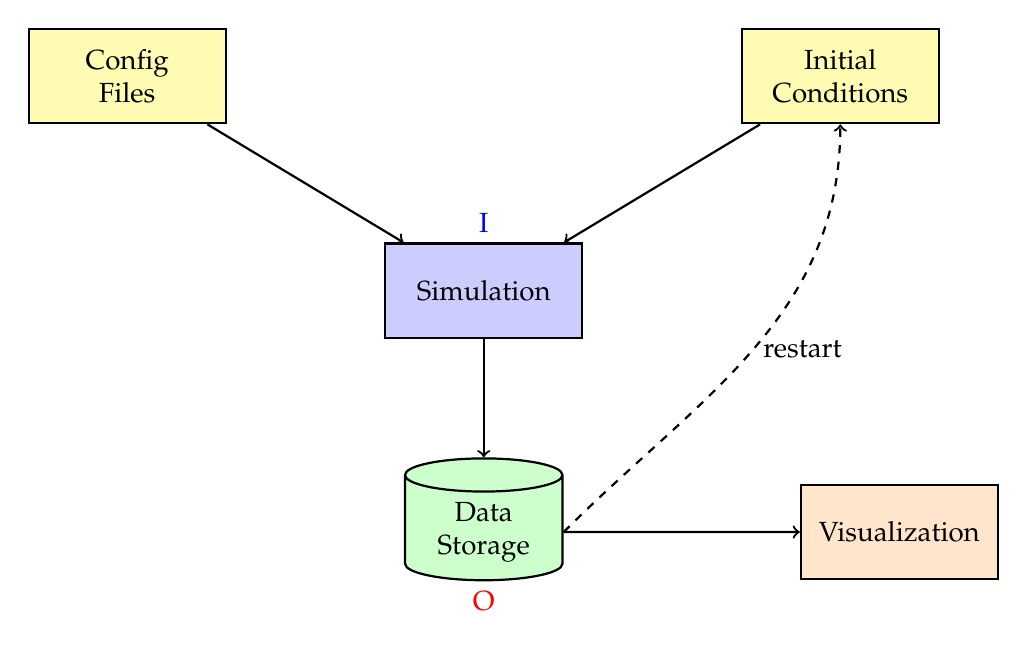
\begin{tikzpicture}[
    node distance=1.5cm and 2cm,
    box/.style={rectangle, draw, thick, minimum width=2.5cm, minimum height=1.2cm, align=center},
    data/.style={cylinder, draw, thick, minimum width=2cm, minimum height=1.5cm, shape border rotate=90, align=center, aspect=0.3}
]
    % Nodes
    \node[box, fill=blue!20] (sim) {Simulation};
    \node[box, fill=yellow!30, above left=of sim] (config) {Config\\Files};
    \node[box, fill=yellow!30, above right=of sim] (initial) {Initial\\Conditions};
    \node[data, fill=green!20, below=of sim] (data) {Data\\Storage};
    \node[box, fill=orange!20, right=3cm of data] (viz) {Visualization};
    
    % Arrows
    \draw[->, thick] (config) -- (sim);
    \draw[->, thick] (initial) -- (sim);
    \draw[->, thick] (sim) -- (data);
    \draw[->, thick] (data) -- (viz);
    \draw[->, thick, dashed] (data.east) to[out=45, in=-90] node[right, pos=0.5] {restart} (initial.south);
    
    % Labels
    \node[above, blue] at (sim.north) {I};
    \node[below, red] at (data.south) {O};
\end{tikzpicture}
\caption{The computational workflow cycle showing I/O relationships.}
\end{figure}

\textbf{Types of I/O in scientific computing}:
\begin{itemize}
\item \textbf{Configuration}: Reading simulation parameters (grid size, time step, etc.)
\item \textbf{Initial conditions}: Starting state of the system
\item \textbf{Checkpointing}: Saving intermediate states for restart capability
\item \textbf{Results}: Outputting computed data for analysis
\item \textbf{Visualization data}: Formatted output for plotting and rendering
\item \textbf{Logging}: Tracking simulation progress and diagnostics
\end{itemize}

\section{Standard Streams in C++}

C++ provides three standard streams for basic I/O operations. These streams are automatically available and connected to the console/terminal by default.

\subsection{The Three Standard Streams}

\subsubsection{Standard Input (stdin)}

\textbf{Stream object}: \texttt{std::cin} (character input)

\textbf{Purpose}: Reading input from the user or from redirected files

\textbf{Syntax}:
\begin{lstlisting}[language=C++]
std::cin >> variable;
\end{lstlisting}

The \texttt{>>} operator is called the \textbf{extraction operator}. It extracts (reads) data from the input stream and stores it in the variable.

\begin{lstlisting}[language=C++, caption={Reading from standard input}]
#include <iostream>

int main() {
    int age;
    std::string name;
    
    std::cout << "Enter your name: ";
    std::cin >> name;  // Reads one word (stops at whitespace)
    
    std::cout << "Enter your age: ";
    std::cin >> age;   // Reads an integer
    
    std::cout << "Hello, " << name << "! You are " 
              << age << " years old.\n";
    
    return 0;
}
\end{lstlisting}

\textbf{Important behavior}: The \texttt{>>} operator skips whitespace (spaces, tabs, newlines) and stops reading at the next whitespace. To read entire lines including spaces, use \texttt{std::getline()}.

\subsubsection{Standard Output (stdout)}

\textbf{Stream object}: \texttt{std::cout} (character output)

\textbf{Purpose}: Writing output to the console/terminal

\textbf{Syntax}:
\begin{lstlisting}[language=C++]
std::cout << value;
\end{lstlisting}

The \texttt{<<} operator is called the \textbf{insertion operator}. It inserts (writes) data to the output stream.

\begin{lstlisting}[language=C++, caption={Writing to standard output}]
#include <iostream>

int main() {
    int x = 42;
    double pi = 3.14159;
    std::string message = "Hello, World!";
    
    // Single output
    std::cout << message;
    
    // Chaining multiple outputs
    std::cout << "x = " << x << ", pi = " << pi << "\n";
    
    // Using std::endl (flushes buffer)
    std::cout << "This is a new line" << std::endl;
    
    return 0;
}
\end{lstlisting}

\textbf{Note on} \texttt{std::endl} vs \texttt{"\textbackslash n"}:
\begin{itemize}
\item \texttt{"\textbackslash n"}: Just adds a newline character (fast)
\item \texttt{std::endl}: Adds a newline AND flushes the output buffer (slower but ensures immediate output)
\end{itemize}

For performance-critical code, prefer \texttt{"\textbackslash n"}. Use \texttt{std::endl} when you need to ensure output appears immediately (e.g., before a crash or long computation).

\subsubsection{Standard Error (stderr)}

\textbf{Stream object}: \texttt{std::cerr} (character error)

\textbf{Purpose}: Writing error messages and diagnostics

\textbf{Syntax}:
\begin{lstlisting}[language=C++]
std::cerr << error_message;
\end{lstlisting}

\begin{lstlisting}[language=C++, caption={Writing to standard error}]
#include <iostream>

int main() {
    int result = some_computation();
    
    if (result < 0) {
        std::cerr << "Error: Computation failed with code " 
                  << result << "\n";
        return 1;  // Return error code
    }
    
    std::cout << "Success: Result = " << result << "\n";
    return 0;  // Return success
}
\end{lstlisting}

\textbf{Why use} \texttt{std::cerr} instead of \texttt{std::cout}?
\begin{itemize}
\item \texttt{std::cerr} is \textbf{unbuffered} (output appears immediately)
\item Separates normal output from error messages
\item Allows redirecting output and errors to different files
\item Standard practice: users expect errors on stderr, results on stdout
\end{itemize}

\subsection{Required Headers}

To use these streams, you must include the appropriate headers:

\begin{lstlisting}[language=C++, caption={Stream headers}]
#include <iostream>  // For std::cin, std::cout, std::cerr
#include <istream>   // For input stream operations (rarely needed directly)
#include <ostream>   // For output stream operations (rarely needed directly)
\end{lstlisting}

In practice, \texttt{<iostream>} is almost always sufficient as it includes the necessary components from \texttt{<istream>} and \texttt{<ostream>}.

\subsection{Stream Objects are Not Copyable}

\textbf{Critical rule}: Stream objects cannot be copied or assigned!

\begin{lstlisting}[language=C++, caption={Stream object constraints}]
// This is ILLEGAL and will not compile:
std::ostream out = std::cout;  // ERROR: No copy constructor

// If you need to pass streams to functions, use references
void write_data(std::ostream& os, int value) {
    os << "Value: " << value << "\n";
}

// Note: reference must be non-const for output operations
void read_data(std::istream& is, int& value) {
    is >> value;
}

int main() {
    int x = 42;
    write_data(std::cout, x);  // Pass by reference
    
    int y;
    read_data(std::cin, y);    // Pass by reference
    
    return 0;
}
\end{lstlisting}

\textbf{Why this restriction?} Streams represent system resources (file handles, console connections) that cannot be duplicated. Copying would lead to ambiguous ownership and resource management issues.

% \begin{figure}[h!]
% \centering
% \includegraphics[width=0.6\textwidth]{placeholder_standard_streams_diagram.png}
% \caption{Diagram showing the three standard streams (stdin, stdout, stderr) and their connection to a program. The diagram illustrates how stream \#0 (stdin) connects to the keyboard, stream \#1 (stdout) connects to the display for normal output, and stream \#2 (stderr) connects to the display for error messages.}
% \label{fig:standard_streams}
% \end{figure}

\begin{figure}[h!]
\centering
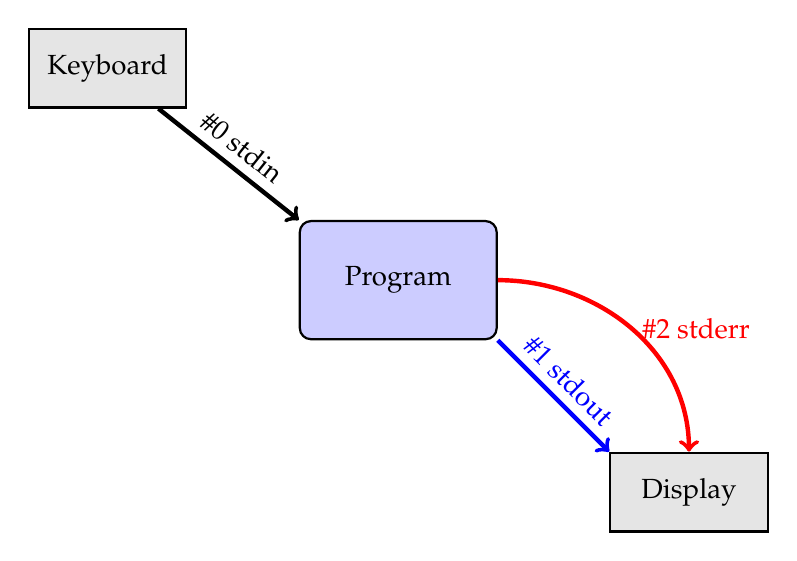
\begin{tikzpicture}[
    node distance=2cm,
    box/.style={rectangle, draw, thick, minimum width=2.5cm, minimum height=1.5cm, align=center, rounded corners},
    device/.style={rectangle, draw, thick, minimum width=2cm, minimum height=1cm, align=center, fill=gray!20}
]
    % Program
    \node[box, fill=blue!20] (prog) {Program};
    
    % Devices
    \node[device, above left=of prog] (keyboard) {Keyboard};
    \node[device, below right=of prog] (display) {Display};
    
    % Streams
    \draw[->, ultra thick] (keyboard) -- node[above, sloped] {\#0 stdin} (prog.north west);
    \draw[->, ultra thick, blue] (prog.south east) -- node[above, sloped] {\#1 stdout} (display.north west);
    \draw[->, ultra thick, red] (prog.east) to[out=0, in=90] node[right] {\#2 stderr} (display.north);
\end{tikzpicture}
\caption{Diagram showing the three standard streams and their connections.}
\end{figure}

\section{Shell Pipelining and Redirection}

The Unix/Linux shell provides powerful mechanisms for connecting programs and redirecting their input/output. These techniques are essential for building flexible, composable scientific computing workflows.

\subsection{Pipelining: Chaining Programs}

A \textbf{pipeline} connects the output of one program directly to the input of another, creating a sequence of data transformations.

\textbf{Syntax (bash)}:
\begin{lstlisting}[language=bash]
$ program1 | program2 | program3
\end{lstlisting}

The pipe operator \texttt{|} connects standard output of one program to standard input of the next.

\textbf{Example}: Count the number of lines containing "error" in a log file:
\begin{lstlisting}[language=bash]
$ cat simulation.log | grep "error" | wc -l
\end{lstlisting}

This pipeline:
\begin{enumerate}
\item \texttt{cat simulation.log}: Outputs file contents to stdout
\item \texttt{grep "error"}: Reads from stdin, outputs lines containing "error"
\item \texttt{wc -l}: Reads from stdin, counts lines
\end{enumerate}

\textbf{Scientific computing example}:
\begin{lstlisting}[language=bash]
$ cat words.txt | ./stdstream2
\end{lstlisting}

If \texttt{stdstream2} is a C++ program that reads from \texttt{std::cin} and processes text, it receives the contents of \texttt{words.txt} as input.

\subsection{Output Redirection}

\textbf{Redirecting standard output to a file}:
\begin{lstlisting}[language=bash]
$ ./stdstream3 > out.log
\end{lstlisting}

This runs \texttt{stdstream3} and saves all stdout to \texttt{out.log} instead of displaying it.

\textbf{Redirecting stdout and stderr separately}:
\begin{lstlisting}[language=bash]
$ ./stdstream3 1> out.log 2> err.log
\end{lstlisting}

\textbf{Syntax explanation}:
\begin{itemize}
\item \texttt{1>}: Redirects file descriptor 1 (stdout)
\item \texttt{2>}: Redirects file descriptor 2 (stderr)
\end{itemize}

\textbf{Redirecting both to the same file}:
\begin{lstlisting}[language=bash]
$ ./stdstream3 &> my.log
\end{lstlisting}

This saves both stdout and stderr to \texttt{my.log}.

\textbf{Alternative syntax (compatible with older shells)}:
\begin{lstlisting}[language=bash]
$ ./stdstream3 2>&1 | less
\end{lstlisting}

This redirects stderr to stdout (\texttt{2>\&1}), then pipes everything to \texttt{less} for viewing.

\subsection{Using a Terminal Pager}

For viewing long output, pipe to a pager like \texttt{less}:

\begin{lstlisting}[language=bash]
# Pipe stdout to less
$ ./stdstream3 | less

# Pipe both stdout and stderr to less (bash version >= 4)
$ ./stdstream3 |& less

# Pipe both stdout and stderr to less (older shells)
$ ./stdstream3 2>&1 | less
\end{lstlisting}

\textbf{Benefits of using a pager}:
\begin{itemize}
\item Scroll through output with keyboard
\item Search for text with \texttt{/pattern}
\item Navigate large outputs efficiently
\item Doesn't fill up terminal with thousands of lines
\end{itemize}

% \begin{figure}[h!]
% \centering
% \includegraphics[width=0.8\textwidth]{placeholder_pipeline_diagram.png}
% \caption{Visualization of shell pipelining showing how multiple programs can be chained together, with the output of each program feeding into the input of the next. The diagram shows three programs connected by pipes, and an alternative configuration where stdout and stderr are redirected to different destinations.}
% \label{fig:pipeline}
% \end{figure}
\begin{figure}[h!]
\centering
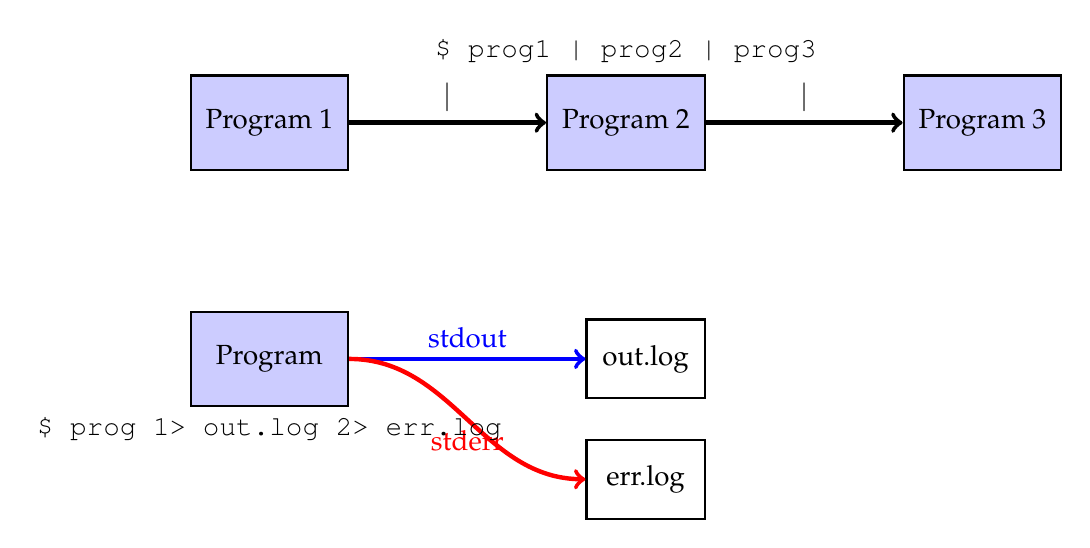
\begin{tikzpicture}[
    node distance=2.5cm,
    box/.style={rectangle, draw, thick, minimum width=2cm, minimum height=1.2cm, align=center, fill=blue!20}
]
    % Pipeline
    \node[box] (p1) {Program 1};
    \node[box, right=of p1] (p2) {Program 2};
    \node[box, right=of p2] (p3) {Program 3};
    
    \draw[->, ultra thick] (p1) -- node[above] {$|$} (p2);
    \draw[->, ultra thick] (p2) -- node[above] {$|$} (p3);
    
    \node[above] at (p2.north) {\texttt{\$ prog1 | prog2 | prog3}};
    
    % Redirection example
    \begin{scope}[yshift=-3cm]
        \node[box] (prog) {Program};
        \node[draw, thick, minimum width=1.5cm, minimum height=1cm, right=3cm of prog] (file1) {out.log};
        \node[draw, thick, minimum width=1.5cm, minimum height=1cm, below=0.5cm of file1] (file2) {err.log};
        
        \draw[->, ultra thick, blue] (prog.east) to[out=0, in=180] node[above] {stdout} (file1.west);
        \draw[->, ultra thick, red] (prog.east) to[out=0, in=180] node[below] {stderr} (file2.west);
        
        \node[below] at (prog.south) {\texttt{\$ prog 1> out.log 2> err.log}};
    \end{scope}
\end{tikzpicture}
\caption{Visualization of shell pipelining and redirection.}
\end{figure}

\textbf{Related material}: See Problem 1.3 in your course materials for a Unix shell tutorial with more detailed examples.

\section{Formatted Output in C++}

By default, C++'s \texttt{<<} operator converts values to "human-readable" text form using reasonable defaults. However, for professional output (especially tables and scientific data), we need precise control over formatting.

\subsection{Default Formatting Behavior}

When you use \texttt{std::cout << value}, C++ applies default formatting rules:

\subsubsection{Integers}

\begin{itemize}
\item All digits are displayed
\item No leading or trailing spaces
\item Decimal base (base 10)
\end{itemize}

\begin{lstlisting}[language=C++, caption={Default integer formatting}]
int x = 12345;
std::cout << x;  // Output: 12345
\end{lstlisting}

\subsubsection{Floating-point Numbers}

\begin{itemize}
\item \textbf{Default precision}: 6 digits total (including digits before and after decimal point, excluding leading zeros)
\item \textbf{Scientific notation}: Used when exponent $\geq 6$ or exponent $\leq -5$
\item Trailing zeros after decimal point are removed
\end{itemize}

\begin{lstlisting}[language=C++, caption={Default floating-point formatting}]
double a = 3.14159265359;
std::cout << a;  // Output: 3.14159 (6 significant digits)

double b = 1234567.89;
std::cout << b;  // Output: 1.23457e+06 (scientific notation)

double c = 0.0000012345;
std::cout << c;  // Output: 1.2345e-06 (scientific notation)
\end{lstlisting}

\subsection{I/O Manipulators}

To control formatting precisely, C++ provides \textbf{I/O manipulators}. These are special functions that modify stream properties.

\textbf{Required headers}:
\begin{lstlisting}[language=C++]
#include <iostream>  // Basic manipulators (std::endl, etc.)
#include <iomanip>   // Advanced manipulators (std::setw, std::setprecision, etc.)
\end{lstlisting}

\subsection{Manipulator Categories: Sticky vs. Non-Sticky}

Understanding manipulator persistence is crucial:

\textbf{Non-sticky manipulators}: Apply only to the \textit{next} output operation, then revert
\begin{itemize}
\item Example: \texttt{std::setw} (field width)
\end{itemize}

\textbf{Sticky manipulators}: Persist for all subsequent operations until explicitly changed
\begin{itemize}
\item Examples: \texttt{std::setfill}, \texttt{std::setprecision}, \texttt{std::fixed}, \texttt{std::left}
\end{itemize}

\subsection{Basic Formatting Manipulators}

\subsubsection{Field Width: setw}

\texttt{std::setw(x)} sets the minimum field width to \texttt{x} characters for the next output.

\textbf{Important}: \texttt{setw} is \textbf{non-sticky}!

\begin{lstlisting}[language=C++, caption={Using setw for field width}]
#include <iostream>
#include <iomanip>

int main() {
    int x = 42;
    
    // Default: no extra spacing
    std::cout << x << "\n";  // Output: 42
    
    // Set width to 10 characters
    std::cout << std::setw(10) << x << "\n";  // Output: "        42"
    
    // setw applies only to next output!
    std::cout << x << "\n";  // Output: 42 (width reset to default)
    
    // Need to reapply for each output
    std::cout << std::setw(10) << x << std::setw(10) << x << "\n";
    // Output: "        42        42"
    
    return 0;
}
\end{lstlisting}

\subsubsection{Fill Character: setfill}

\texttt{std::setfill(c)} sets the character used to pad fields to the specified width.

\textbf{Important}: \texttt{setfill} is \textbf{sticky}!

\begin{lstlisting}[language=C++, caption={Using setfill for padding}]
#include <iostream>
#include <iomanip>

int main() {
    int x = 42;
    
    // Default fill character is space
    std::cout << std::setw(10) << x << "\n";  // Output: "        42"
    
    // Change fill character to '0' (sticky!)
    std::cout << std::setfill('0');
    std::cout << std::setw(10) << x << "\n";  // Output: "0000000042"
    
    // Fill character persists
    std::cout << std::setw(8) << x << "\n";   // Output: "00000042"
    
    // Change fill character to '#'
    std::cout << std::setfill('#');
    std::cout << std::setw(10) << x << "\n";  // Output: "########42"
    
    return 0;
}
\end{lstlisting}

\subsubsection{Alignment: left, right, internal}

These manipulators control how values are aligned within their field width.

\textbf{Important}: These are \textbf{sticky}!

\begin{lstlisting}[language=C++, caption={Alignment manipulators}]
#include <iostream>
#include <iomanip>

int main() {
    int x = 42;
    
    // Default is right-aligned
    std::cout << std::setw(10) << x << "\n";  // "        42"
    
    // Left-aligned (sticky!)
    std::cout << std::left;
    std::cout << std::setw(10) << x << "\n";  // "42        "
    
    // Still left-aligned
    std::cout << std::setw(10) << x << "\n";  // "42        "
    
    // Back to right-aligned
    std::cout << std::right;
    std::cout << std::setw(10) << x << "\n";  // "        42"
    
    // Internal alignment (for numbers with signs)
    std::cout << std::setfill('*') << std::internal;
    std::cout << std::setw(10) << -42 << "\n";  // "-*******42"
    
    return 0;
}
\end{lstlisting}

\subsection{Floating-Point Formatting}

\subsubsection{Precision: setprecision}

\texttt{std::setprecision(x)} sets the precision for floating-point output.

\textbf{Important}: \texttt{setprecision} is \textbf{sticky}!

The meaning of "precision" depends on the format mode:
\begin{itemize}
\item \textbf{Default mode}: Number of significant digits (total)
\item \textbf{Fixed mode}: Number of digits after decimal point
\item \textbf{Scientific mode}: Number of digits after decimal point
\end{itemize}

\begin{lstlisting}[language=C++, caption={Using setprecision}]
#include <iostream>
#include <iomanip>

int main() {
    double pi = 3.14159265359;
    
    // Default: 6 significant digits
    std::cout << pi << "\n";  // 3.14159
    
    // Change precision to 10 (sticky!)
    std::cout << std::setprecision(10);
    std::cout << pi << "\n";  // 3.141592654
    
    // Still 10 significant digits
    std::cout << pi * 1000 << "\n";  // 3141.592654
    
    return 0;
}
\end{lstlisting}

\subsubsection{Format Modes: fixed, scientific, defaultfloat}

These manipulators control how floating-point numbers are displayed.

\textbf{Important}: These are \textbf{sticky}!

\begin{lstlisting}[language=C++, caption={Floating-point format modes}]
#include <iostream>
#include <iomanip>

int main() {
    double x = 12345.6789;
    
    // Default mode (switches to scientific for large/small numbers)
    std::cout << x << "\n";  // 12345.7 (6 significant digits)
    
    // Fixed mode: always show decimal point
    std::cout << std::fixed << std::setprecision(2);
    std::cout << x << "\n";  // 12345.68 (2 digits after decimal)
    
    // Scientific notation
    std::cout << std::scientific << std::setprecision(4);
    std::cout << x << "\n";  // 1.2346e+04 (4 digits after decimal)
    
    // Back to default (C++11)
    std::cout << std::defaultfloat << std::setprecision(6);
    std::cout << x << "\n";  // 12345.7
    
    return 0;
}
\end{lstlisting}

\subsection{Complete Formatted Table Example}

Here's a complete example demonstrating formatted table output:

\begin{lstlisting}[language=C++, caption={Creating a formatted table}]
#include <iostream>
#include <iomanip>
#include <cmath>

int main() {
    std::cout << std::fixed << std::setprecision(4);
    std::cout << std::setfill(' ');
    
    // Header
    std::cout << std::left;
    std::cout << std::setw(10) << "x"
              << std::setw(15) << "sin(x)"
              << std::setw(15) << "cos(x)"
              << std::setw(15) << "tan(x)" << "\n";
    
    // Separator
    std::cout << std::setfill('-');
    std::cout << std::setw(55) << "" << "\n";
    std::cout << std::setfill(' ');
    
    // Data rows
    std::cout << std::right;
    for (int i = 0; i <= 6; ++i) {
        double x = i * M_PI / 6.0;
        std::cout << std::setw(10) << x
                  << std::setw(15) << std::sin(x)
                  << std::setw(15) << std::cos(x)
                  << std::setw(15) << std::tan(x) << "\n";
    }
    
    return 0;
}
\end{lstlisting}

\textbf{Output}:
\begin{verbatim}
x         sin(x)         cos(x)         tan(x)         
-------------------------------------------------------
   0.0000        0.0000        1.0000        0.0000
   0.5236        0.5000        0.8660        0.5774
   1.0472        0.8660        0.5000        1.7321
   1.5708        1.0000        0.0000    Inf (or very large)
   ...
\end{verbatim}

\subsection{Modern C++ Formatting (C++20/23)}

C++20 introduced \texttt{std::format} and C++23 added \texttt{std::print}, providing Python-style formatting:

\begin{lstlisting}[language=C++, caption={Modern formatting with C++20/23}]
#include <iostream>
#include <format>  // C++20
#include <print>   // C++23

int main() {
    int x = 42;
    double pi = 3.14159;
    
    // C++20: std::format (returns string)
    std::string s = std::format("x = {}, pi = {:.2f}", x, pi);
    std::cout << s << "\n";  // x = 42, pi = 3.14
    
    // C++23: std::print (directly outputs)
    std::print("x = {}, pi = {:.2f}\n", x, pi);
    
    // Positional arguments
    std::print("{1} comes before {0}\n", "second", "first");
    // Output: first comes before second
    
    // Named arguments (C++23)
    std::print("My name is {name} and I'm {age} years old\n",
               .name = "Alice", .age = 30);
    
    return 0;
}
\end{lstlisting}

These modern features are more concise and less error-prone than traditional manipulators.

\textbf{Documentation}: For complete details on all manipulators, see the C++ standard library documentation for \texttt{<iomanip>}.

\section{String Streams: Reading and Writing Strings}

\textbf{String streams} allow you to perform formatted I/O operations on strings, just as you would with files or console I/O. This is incredibly useful for:
\begin{itemize}
\item Generating formatted file names
\item Parsing structured text data
\item Building complex strings piece by piece
\item Converting between types and strings
\end{itemize}

\subsection{Header and Stream Types}

\begin{lstlisting}[language=C++]
#include <sstream>  // Required header

// Three types of string streams:
std::istringstream  // Input string stream (reading from strings)
std::ostringstream  // Output string stream (writing to strings)  
std::stringstream   // Bidirectional string stream (reading and writing)
\end{lstlisting}

\subsection{Writing to Strings with ostringstream}

\texttt{std::ostringstream} lets you build strings using the familiar \texttt{<<} operator:

\begin{lstlisting}[language=C++, caption={Writing to strings}]
#include <iostream>
#include <sstream>
#include <iomanip>

int main() {
    std::ostringstream ss;
    
    // Write formatted data to string stream
    ss << std::setw(5) << std::setfill('0') << 42;
    
    // Extract the string
    std::string s = ss.str();
    
    std::cout << s << "\n";  // Output: 00042
    
    return 0;
}
\end{lstlisting}

\subsection{Practical Example: Generating File Names}

A common use case in scientific computing is generating numbered file names for simulation output:

\begin{lstlisting}[language=C++, caption={Generating numbered file names}]
#include <iostream>
#include <sstream>
#include <iomanip>
#include <fstream>

// Function to generate filename with zero-padded number
std::string make_filename(const std::string& prefix, 
                          int number, 
                          const std::string& extension) {
    std::ostringstream ss;
    ss << prefix 
       << std::setw(5) << std::setfill('0') << number 
       << extension;
    return ss.str();
}

int main() {
    // Generate file names for time steps
    for (int step = 0; step <= 100; ++step) {
        std::string filename = make_filename("out", step, ".dat");
        std::cout << filename << "\n";
        
        // In real code, you would write data to this file:
        // std::ofstream file(filename);
        // file << data;
    }
    
    return 0;
}
\end{lstlisting}

\textbf{Output}:
\begin{verbatim}
out00000.dat
out00001.dat
out00002.dat
...
out00099.dat
out00100.dat
\end{verbatim}

\textbf{Why zero-padding?} Files with zero-padded numbers sort correctly:
\begin{itemize}
\item Good: \texttt{out00001.dat, out00002.dat, ..., out00010.dat}
\item Bad: \texttt{out1.dat, out10.dat, out2.dat, ...} (lexicographic sorting fails)
\end{itemize}

\subsection{Reading from Strings with istringstream}

\texttt{std::istringstream} allows parsing formatted data from strings:

\begin{lstlisting}[language=C++, caption={Parsing data from strings}]
#include <iostream>
#include <sstream>
#include <string>

int main() {
    std::string data = "42 3.14 Hello";
    
    std::istringstream iss(data);
    
    int integer;
    double floating;
    std::string word;
    
    // Extract values using >> operator
    iss >> integer >> floating >> word;
    
    std::cout << "Integer: " << integer << "\n";
    std::cout << "Floating: " << floating << "\n";
    std::cout << "Word: " << word << "\n";
    
    return 0;
}
\end{lstlisting}

This is particularly useful for parsing configuration files or command-line arguments.

\subsection{Bidirectional String Streams}

\texttt{std::stringstream} combines input and output capabilities:

\begin{lstlisting}[language=C++, caption={Bidirectional string stream}]
#include <iostream>
#include <sstream>

int main() {
    std::stringstream ss;
    
    // Write to stream
    ss << 42 << " " << 3.14;
    
    // Read from same stream
    int x;
    double y;
    ss >> x >> y;
    
    std::cout << "Read: x=" << x << ", y=" << y << "\n";
    
    return 0;
}
\end{lstlisting}

% \begin{figure}[h!]
% \centering
% \includegraphics[width=0.7\textwidth]{placeholder_string_stream_example.png}
% \caption{Visual example showing generated file names with zero-padding (out00000.dat, out00001.dat, etc.) demonstrating proper lexicographic sorting of output files.}
% \label{fig:string_stream}
% \end{figure}

\begin{figure}[h!]
\centering
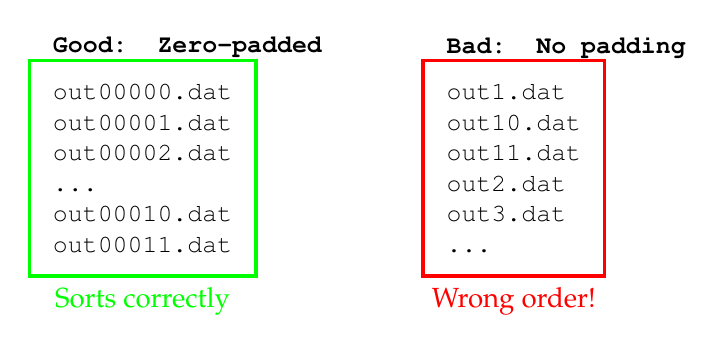
\begin{tikzpicture}
    % Good example
    \node[anchor=north west, font=\ttfamily\small] (good_title) at (0,0) {\textbf{Good: Zero-padded}};
    \node[anchor=north west, font=\ttfamily\small, align=left] (good_list) at (0,-0.6) {
        out00000.dat\\
        out00001.dat\\
        out00002.dat\\
        \ldots\\
        out00010.dat\\
        out00011.dat
    };
    
    % Bad example
    \node[anchor=north west, font=\ttfamily\small] (bad_title) at (5,0) {\textbf{Bad: No padding}};
    \node[anchor=north west, font=\ttfamily\small, align=left] (bad_list) at (5,-0.6) {
        out1.dat\\
        out10.dat\\
        out11.dat\\
        out2.dat\\
        out3.dat\\
        \ldots
    };
    
    % Annotations
    \node[draw=green, very thick, fit=(good_list), inner sep=5pt] (good_box) {};
    \node[green, below] at (good_box.south) {Sorts correctly};
    
    \node[draw=red, very thick, fit=(bad_list), inner sep=5pt] (bad_box) {};
    \node[red, below] at (bad_box.south) {Wrong order!};
\end{tikzpicture}
\caption{File naming with and without zero-padding.}
\end{figure}

\section{File Streams: Reading and Writing Files}

File I/O in C++ follows the same pattern as standard streams, but with additional setup for opening and closing files.

\subsection{File Stream Classes}

\begin{lstlisting}[language=C++]
#include <fstream>  // Required header

// Three file stream classes:
std::ifstream  // Input file stream (reading from files)
std::ofstream  // Output file stream (writing to files)
std::fstream   // Bidirectional file stream (reading and writing)
\end{lstlisting}

\subsection{Basic File Output Workflow}

\textbf{Steps for writing to a file}:
\begin{enumerate}
\item Construct an \texttt{ofstream} object
\item Connect the stream to a file (open) and set the mode
\item Perform output operations using \texttt{<<} or \texttt{write()}
\item Close the stream (happens automatically when object is destroyed)
\end{enumerate}

\begin{lstlisting}[language=C++, caption={Writing to a file}]
#include <fstream>
#include <iostream>

int main() {
    // Create and open file in one step
    std::ofstream outfile("output.txt");
    
    // Check if file opened successfully
    if (!outfile) {
        std::cerr << "Error: Could not open file\n";
        return 1;
    }
    
    // Write to file just like cout
    outfile << "Hello, file!\n";
    outfile << "x = " << 42 << "\n";
    outfile << "pi = " << 3.14159 << "\n";
    
    // File automatically closed when outfile goes out of scope
    return 0;
}
\end{lstlisting}

\subsection{Basic File Input Workflow}

\textbf{Steps for reading from a file}:
\begin{enumerate}
\item Construct an \texttt{ifstream} object
\item Connect the stream to a file (open) and set the mode
\item Perform input operations using \texttt{>>}, \texttt{getline()}, or \texttt{read()}
\item Close the stream (happens automatically when object is destroyed)
\end{enumerate}

\begin{lstlisting}[language=C++, caption={Reading from a file}]
#include <fstream>
#include <iostream>
#include <string>

int main() {
    // Open file for reading
    std::ifstream infile("input.txt");
    
    // Check if file opened successfully
    if (!infile) {
        std::cerr << "Error: Could not open file\n";
        return 1;
    }
    
    // Read data
    int x;
    double y;
    std::string line;
    
    infile >> x >> y;              // Formatted input
    std::getline(infile, line);    // Read entire line
    
    std::cout << "Read: x=" << x << ", y=" << y << "\n";
    std::cout << "Line: " << line << "\n";
    
    // File automatically closed
    return 0;
}
\end{lstlisting}

\subsection{File Modes}

File modes control how files are opened and accessed. They are specified as bit flags that can be combined using the bitwise OR operator \texttt{|}.

\textbf{Available file modes (from} \texttt{std::fstream} class\textbf{)}:

\begin{itemize}
\item \texttt{std::fstream::in}: Open for input (reading)
\item \texttt{std::fstream::out}: Open for output (writing)
\item \texttt{std::fstream::binary}: Binary mode (as opposed to text mode)
\item \texttt{std::fstream::ate}: Start at end of file (AT End)
\item \texttt{std::fstream::app}: Append to end of file (all writes go to end)
\item \texttt{std::fstream::trunc}: Truncate file (erase existing content) if it exists
\end{itemize}

\textbf{Mode combinations}:

\begin{lstlisting}[language=C++, caption={File mode examples}]
#include <fstream>

int main() {
    // Write mode (truncates existing file)
    std::ofstream out1("file.txt", std::fstream::out);
    
    // Append mode (preserves existing content)
    std::ofstream out2("file.txt", std::fstream::out | std::fstream::app);
    
    // Binary output mode
    std::ofstream out3("data.bin", std::fstream::out | std::fstream::binary);
    
    // Read-write mode
    std::fstream file("data.dat", std::fstream::in | std::fstream::out);
    
    return 0;
}
\end{lstlisting}

\textbf{Important}: Using \texttt{std::fstream::out} alone typically truncates the file! To preserve existing content while writing, use \texttt{std::fstream::app}.

\subsection{Binary (Unformatted) File I/O}

For efficiency, scientific data is often stored in binary format:

\begin{lstlisting}[language=C++, caption={Binary file output}]
#include <fstream>
#include <vector>

int main() {
    std::vector<double> data = {1.0, 2.0, 3.0, 4.0, 5.0};
    
    // Open file in binary mode
    std::ofstream outfile("data.bin", std::fstream::binary);
    
    // Write binary data
    outfile.write(reinterpret_cast<const char*>(data.data()),
                  data.size() * sizeof(double));
    
    outfile.close();
    
    return 0;
}
\end{lstlisting}

\begin{lstlisting}[language=C++, caption={Binary file input}]
#include <fstream>
#include <vector>
#include <iostream>

int main() {
    std::vector<double> data(5);  // Preallocate space
    
    // Open file in binary mode
    std::ifstream infile("data.bin", std::fstream::binary);
    
    // Read binary data
    infile.read(reinterpret_cast<char*>(data.data()),
                data.size() * sizeof(double));
    
    // Display
    for (double val : data) {
        std::cout << val << " ";
    }
    std::cout << "\n";
    
    return 0;
}
\end{lstlisting}

\textbf{Binary I/O is useful for}:
\begin{itemize}
\item Large datasets (more compact than text)
\item Faster I/O (no text conversion)
\item Preserving exact floating-point values
\end{itemize}

\textbf{BUT} binary files have issues (discussed in next section)!

\section{Issues with Binary Files}

While binary files are efficient, they have significant drawbacks for scientific computing that must be understood.

\subsection{The File Format Problem}

\textbf{File format} refers to information about the data layout—specifically, how the data is stored in the file.

\textbf{The fundamental problem}: To read a binary file, you must know its format!

Binary files contain raw bytes with no inherent structure. Without documentation, a binary file is essentially meaningless data. Consider:
\begin{itemize}
\item How many variables are stored?
\item What are their types? (int, float, double?)
\item What are their dimensions? (scalar, 1D array, 2D array?)
\item In what order are they stored?
\item What do they represent physically?
\end{itemize}

\textbf{Example scenario}: You create a simulation that writes binary output:
\begin{lstlisting}[language=C++]
// Your program writes:
int nx = 100, ny = 100;
std::vector<double> temperature(nx * ny);
std::vector<double> pressure(nx * ny);

outfile.write(reinterpret_cast<char*>(&nx), sizeof(int));
outfile.write(reinterpret_cast<char*>(&ny), sizeof(int));
outfile.write(reinterpret_cast<char*>(temperature.data()), 
              temperature.size() * sizeof(double));
outfile.write(reinterpret_cast<char*>(pressure.data()), 
              pressure.size() * sizeof(double));
\end{lstlisting}

Five years later, you want to analyze the data. Questions:
\begin{itemize}
\item Did you store nx and ny?
\item Were they int or size\_t?
\item Did temperature come before pressure or after?
\item Were there other fields you forgot about?
\item Do you still have the source code to check?
\end{itemize}

\textbf{Real-world consequence}: Scientific results become unreproducible if you cannot read your own old data!

\subsection{Portability Issues}

Even if you know the format, binary files have portability problems:

\subsubsection{Endianness}

\textbf{Endianness} refers to the byte order used to store multi-byte values.

\begin{itemize}
\item \textbf{Little-endian}: Least significant byte stored first (x86, x86-64 processors)
\item \textbf{Big-endian}: Most significant byte stored first (some ARM, historical systems)
\end{itemize}

\textbf{Example}: The 32-bit integer 0x01020304 is stored as:
\begin{itemize}
\item Little-endian: 04 03 02 01 (in memory/file)
\item Big-endian: 01 02 03 04 (in memory/file)
\end{itemize}

If you write a binary file on a little-endian system and read it on a big-endian system (or vice versa), the values will be corrupted!

\subsubsection{Data Type Sizes}

The size of data types can vary between systems:
\begin{itemize}
\item \texttt{int} might be 32 bits or 64 bits
\item \texttt{long} varies (32 bits on Windows, 64 bits on Linux)
\item Floating-point formats can differ
\end{itemize}

\subsubsection{Signed Integer Representation}

Although rare today, historical systems used different representations for negative integers (two's complement vs. one's complement vs. sign-magnitude).

\subsection{Time-Based Issues}

\textbf{Question}: Will you be able to reproduce your scientific results 5, 10, or 20 years from now?

Challenges that arise over time:
\begin{itemize}
\item \textbf{Lost documentation}: Do you still remember the file format?
\item \textbf{Lost source code}: Can you find the program that wrote the files?
\item \textbf{Format confusion}: Did you use a consistent format across all files?
\item \textbf{System changes}: Compilers, hardware, and operating systems evolve
\item \textbf{Colleague dependency}: What if someone else needs to use your data?
\end{itemize}

\textbf{Scientific responsibility}: Reproducibility is a cornerstone of science. If you cannot reproduce your own results due to data access issues, the scientific value is lost.

\subsection{The Solution: Self-Describing Formats}

The solution to these problems is to use \textbf{self-describing, machine-independent data formats}:

\begin{itemize}
\item \textbf{Self-describing}: The file contains metadata about its own structure
\item \textbf{Machine-independent}: Handles endianness and type size differences automatically
\item \textbf{Standardized}: Well-documented, widely supported formats
\end{itemize}

\textbf{Popular formats for scientific computing}:
\begin{itemize}
\item \textbf{HDF5} (Hierarchical Data Format 5): Covered in detail below
\item \textbf{NetCDF}: Popular in climate science and earth sciences
\item \textbf{ASDF} (Advanced Scientific Data Format): Astronomy
\item \textbf{Zarr}: Cloud-optimized array storage
\end{itemize}

\section{HDF5: Hierarchical Data Format 5}

\subsection{Introduction to HDF5}

\textbf{HDF5} is a file format and library designed specifically for storing and managing large, complex scientific data. It has become a de facto standard in many fields of computational science.

\subsubsection{Key Features}

\textbf{Open file format}:
\begin{itemize}
\item Freely available specification
\item No proprietary restrictions
\item Supported by major funding agencies and institutions
\end{itemize}

\textbf{Portable and self-describing}:
\begin{itemize}
\item Files are platform-independent (handles endianness, etc.)
\item Metadata stored within the file itself
\item Files are self-documenting
\end{itemize}

\textbf{Designed for high-volume data}:
\begin{itemize}
\item Efficient storage and access patterns
\item Handles datasets from KB to PB scale
\item Optimized for scientific workloads
\end{itemize}

\textbf{Wide language support}:
\begin{itemize}
\item C/C++/Fortran APIs (native)
\item Python (h5py), MATLAB, R, Julia, IDL
\item Many analysis and visualization tools support HDF5 natively
\end{itemize}

\textbf{Compression}:
\begin{itemize}
\item Built-in compression support (gzip, etc.)
\item Can significantly reduce file sizes
\item Transparent to the user
\end{itemize}

\textbf{Parallel I/O}:
\begin{itemize}
\item Multiple processes can read/write simultaneously
\item Essential for large-scale HPC applications
\item Requires parallel HDF5 build and MPI
\end{itemize}

\subsection{HDF5 Conceptual Model}

At its simplest, HDF5 is a \textbf{data container} that holds data objects in a hierarchical structure, similar to a file system.

\textbf{Simple mental model}: Think of an HDF5 file as a miniature file system contained within a single file on disk. It has "directories" (groups) and "files" (datasets).

% \begin{figure}[h!]
% \centering
% \includegraphics[width=0.8\textwidth]{placeholder_hdf5_objects.png}
% \caption{Overview of HDF5 objects showing the relationship between File, Groups, Datasets, Attributes, Links, Datatypes, Dataspaces, and Property Lists. The diagram illustrates how these components work together to form the HDF5 data model.}
% \label{fig:hdf5_objects}
% \end{figure}

\begin{figure}[h!]
\centering
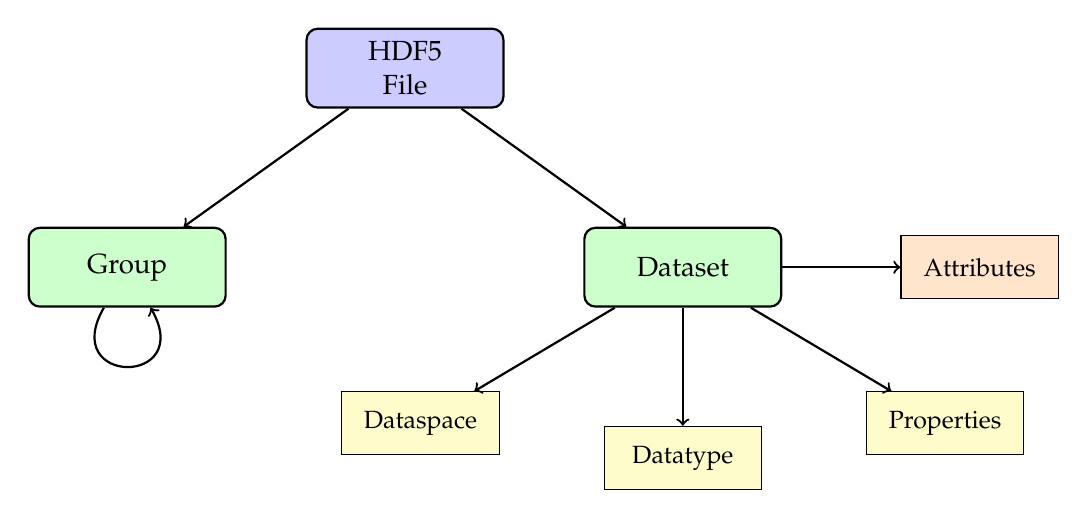
\begin{tikzpicture}[
    node distance=1.5cm,
    box/.style={rectangle, draw, thick, minimum width=2.5cm, minimum height=1cm, align=center, rounded corners},
    smallbox/.style={rectangle, draw, minimum width=2cm, minimum height=0.8cm, align=center, font=\small}
]
    % File
    \node[box, fill=blue!20] (file) {HDF5\\File};
    
    % Primary objects
    \node[box, fill=green!20, below left=1.5cm and 1cm of file] (group) {Group};
    \node[box, fill=green!20, below right=1.5cm and 1cm of file] (dataset) {Dataset};
    
    % Supporting objects
    \node[smallbox, fill=yellow!20, below left=of dataset] (dataspace) {Dataspace};
    \node[smallbox, fill=yellow!20, below=of dataset] (datatype) {Datatype};
    \node[smallbox, fill=yellow!20, below right=of dataset] (properties) {Properties};
    \node[smallbox, fill=orange!20, right=of dataset] (attributes) {Attributes};
    
    % Connections
    \draw[->, thick] (file) -- (group);
    \draw[->, thick] (file) -- (dataset);
    \draw[->, thick] (group) to[out=240, in=300, looseness=5] (group);
    \draw[->, thick] (dataset) -- (dataspace);
    \draw[->, thick] (dataset) -- (datatype);
    \draw[->, thick] (dataset) -- (properties);
    \draw[->, thick] (dataset) -- (attributes);
\end{tikzpicture}
\caption{Overview of HDF5 objects and their relationships.}
\end{figure}

\subsection{HDF5 Primary Objects}

\subsubsection{Groups}

\textbf{Groups} provide the organizational structure for HDF5 files. They are analogous to directories in a file system.

\begin{itemize}
\item \textbf{Purpose}: Organize datasets into a hierarchical structure
\item \textbf{Analogy}: Like folders/directories in a file system
\item \textbf{Root group}: Every HDF5 file has a root group \texttt{/}
\item \textbf{Nesting}: Groups can contain other groups
\item \textbf{Paths}: Objects accessed using Unix-like paths: \texttt{/group1/group2/dataset}
\end{itemize}

\textbf{Example hierarchy}:
\begin{verbatim}
/                          (root group)
├── simulation_parameters/
│   ├── grid_size
│   ├── time_step
│   └── boundary_conditions/
│       ├── left
│       └── right
├── results/
│   ├── temperature
│   ├── pressure
│   └── velocity
└── metadata
    ├── creation_date
    └── author
\end{verbatim}

% \begin{figure}[h!]
% \centering
% \includegraphics[width=0.8\textwidth]{placeholder_hdf5_hierarchy.png}
% \caption{Example HDF5 file structure showing hierarchical organization with groups (Viz, SimOut) and datasets. The diagram illustrates how data is organized in a tree-like structure with the root group at the top, visualization data in one branch, and simulation output data in another.}
% \label{fig:hdf5_hierarchy}
% \end{figure}
\begin{figure}[h!]
\centering
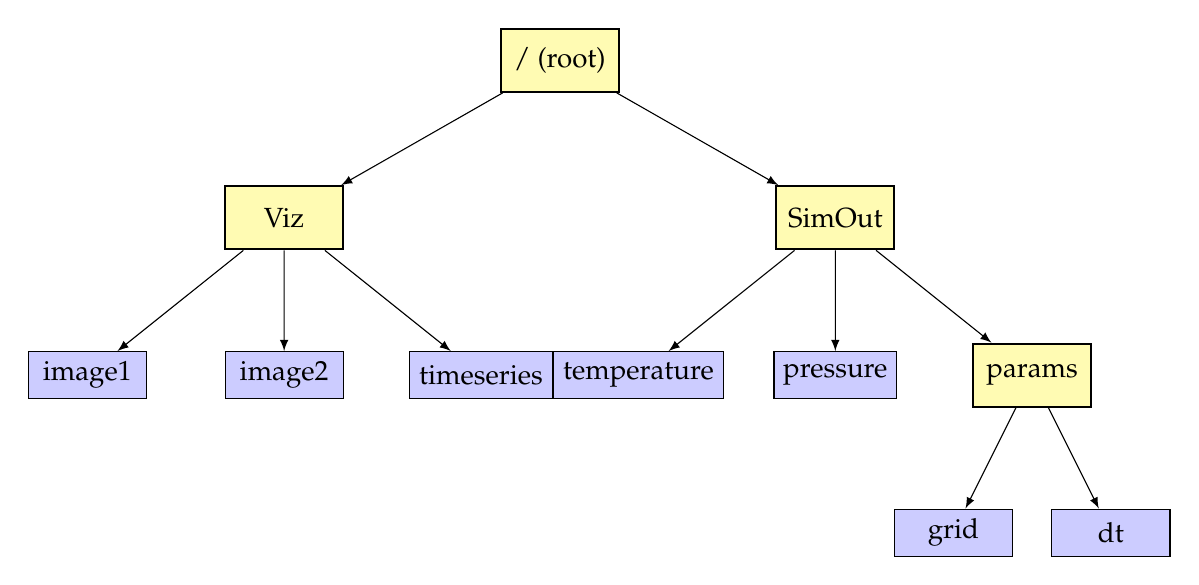
\begin{tikzpicture}[
    grow=south,
    level distance=2cm,
    level 1/.style={sibling distance=7cm},
    level 2/.style={sibling distance=2.5cm},
    level 3/.style={sibling distance=2cm},
    edge from parent/.style={draw, -latex},
    folder/.style={draw, thick, minimum width=1.5cm, minimum height=0.8cm, fill=yellow!30},
    file/.style={draw, minimum width=1.5cm, minimum height=0.6cm, fill=blue!20}
]
    \node[folder] {/ (root)}
        child {node[folder] {Viz}
            child {node[file] {image1}}
            child {node[file] {image2}}
            child {node[file] {timeseries}}
        }
        child {node[folder] {SimOut}
            child {node[file] {temperature}}
            child {node[file] {pressure}}
            child {node[folder] {params}
                child {node[file] {grid}}
                child {node[file] {dt}}
            }
        };
\end{tikzpicture}
\caption{Example HDF5 file structure showing hierarchical organization.}
\end{figure}

\subsubsection{Datasets}

\textbf{Datasets} are the actual data arrays stored in the file.

\begin{itemize}
\item \textbf{Purpose}: Store multidimensional arrays of data
\item \textbf{Structure}: Combination of data + metadata
\item \textbf{Metadata components}:
  \begin{itemize}
  \item \textbf{Dataspace}: Describes the dimensionality and size
  \item \textbf{Datatype}: Specifies the type of elements (int, float, etc.)
  \item \textbf{Properties}: Storage layout, compression, chunking, etc.
  \end{itemize}
\item \textbf{Attributes}: Additional metadata can be attached to datasets
\end{itemize}

% \begin{figure}[h!]
% \centering
% \includegraphics[width=0.9\textwidth]{placeholder_hdf5_dataset.png}
% \caption{Detailed view of an HDF5 dataset showing the three main components: Metadata (including Dataspace with rank and dimensions, Datatype, Attributes, and Properties), and the actual Data array. The diagram illustrates how a dataset encapsulates both the array data and all information needed to interpret it correctly.}
% \label{fig:hdf5_dataset}
% \end{figure}
\begin{figure}[h!]
\centering
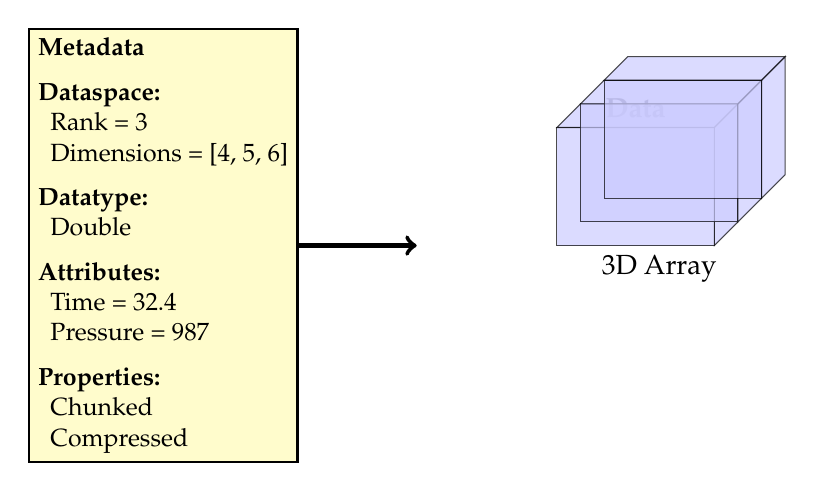
\begin{tikzpicture}[
    node distance=0.3cm,
    box/.style={rectangle, draw, thick, minimum width=3cm, align=left, font=\small}
]
    % Metadata box
    \node[box, fill=yellow!20, minimum height=5cm] (metadata) at (0,0) {
        \textbf{Metadata}\\[5pt]
        \textbf{Dataspace:}\\
        \ \ Rank = 3\\
        \ \ Dimensions = [4, 5, 6]\\[5pt]
        \textbf{Datatype:}\\
        \ \ Double\\[5pt]
        \textbf{Attributes:}\\
        \ \ Time = 32.4\\
        \ \ Pressure = 987\\[5pt]
        \textbf{Properties:}\\
        \ \ Chunked\\
        \ \ Compressed
    };
    
    % Data visualization
    \begin{scope}[xshift=5cm]
        \node[above] at (1, 1.5) {\textbf{Data}};
        % Draw 3D array representation
        \foreach \z in {0, 0.3, 0.6} {
            \draw[fill=blue!20, opacity=0.7] 
                (0+\z, 0+\z) rectangle (2+\z, 1.5+\z);
            \draw[fill=blue!20, opacity=0.7] 
                (2+\z, 0+\z) -- (2.3+\z, 0.3+\z) -- (2.3+\z, 1.8+\z) -- (2+\z, 1.5+\z) -- cycle;
            \draw[fill=blue!20, opacity=0.7] 
                (0+\z, 1.5+\z) -- (0.3+\z, 1.8+\z) -- (2.3+\z, 1.8+\z) -- (2+\z, 1.5+\z) -- cycle;
        }
        \node[below] at (1.3, 0) {3D Array};
    \end{scope}
    
    % Arrow
    \draw[->, ultra thick] (metadata.east) -- ++(1.5, 0);
\end{tikzpicture}
\caption{Detailed view of an HDF5 dataset showing metadata and data components.}
\end{figure}

\subsection{HDF5 Supporting Concepts}

\subsubsection{Dataspace}

\textbf{Dataspace} describes the layout and dimensionality of a dataset's data elements.

\textbf{Two roles}:
\begin{enumerate}
\item \textbf{File dataspace}: Describes how data is laid out in the file
\item \textbf{Memory dataspace}: Describes how data is laid out in memory (during I/O operations)
\end{enumerate}

\textbf{Example}: A 4×6 array in a file

\begin{lstlisting}[language=C++, caption={Dataspace concept}]
// File dataspace
Rank = 2
Dimensions = [4, 6]  // 4 rows, 6 columns
\end{lstlisting}

\begin{figure}[h!]
\centering
\includegraphics[width=0.8\textwidth]{placeholder_hdf5_dataspace_full.png}
\caption{Visual representation of a 4×6 dataspace showing the complete rectangular grid of data elements organized in rows and columns.}
\label{fig:dataspace_full}
\end{figure}

\textbf{Hyperslab selection}: You can select subsets of data using dataspaces

\begin{figure}[h!]
\centering
\includegraphics[width=0.8\textwidth]{placeholder_hdf5_dataspace_selection.png}
\caption{Hyperslab selection showing a subset of the full dataspace highlighted, demonstrating HDF5's ability to read/write partial datasets efficiently without loading the entire array.}
\label{fig:dataspace_selection}
\end{figure}

\begin{figure}[h!]
\centering
\includegraphics[width=0.8\textwidth]{placeholder_hdf5_dataspace_transfer.png}
\caption{Transfer between file and memory showing how a selected region from the file dataspace is read into a corresponding region in the memory buffer, illustrating the flexibility of HDF5 I/O operations.}
\label{fig:dataspace_transfer}
\end{figure}

This allows efficient reading/writing of array slices without loading entire datasets!

\subsubsection{Datatype}

\textbf{Datatypes} describe the individual data elements in a dataset.

\textbf{Standard datatypes} (same on all platforms):
\begin{itemize}
\item \texttt{H5T\_STD\_I32LE}: 32-bit integer, little-endian
\item \texttt{H5T\_IEEE\_F32LE}: 32-bit float, little-endian, IEEE format
\item \texttt{H5T\_IEEE\_F64LE}: 64-bit float (double), little-endian, IEEE format
\end{itemize}

\textbf{Native datatypes} (platform-specific, but converted automatically):
\begin{itemize}
\item \texttt{H5T\_NATIVE\_INT}: Native int (size varies by platform)
\item \texttt{H5T\_NATIVE\_FLOAT}: Native float
\item \texttt{H5T\_NATIVE\_DOUBLE}: Native double
\end{itemize}

\textbf{Derived datatypes}:
\begin{itemize}
\item \textbf{Compound types}: Like C structs
\item \textbf{Array types}: Fixed-size arrays
\item \textbf{Variable-length types}: Dynamic arrays, strings
\end{itemize}

HDF5 automatically handles conversion between different datatypes and platforms, solving the portability problems of raw binary files!

\subsubsection{Properties}

\textbf{Properties} control various aspects of HDF5 objects, especially storage characteristics.

\textbf{Common property settings}:
\begin{itemize}
\item \textbf{Storage layout}:
  \begin{itemize}
  \item Contiguous: Data stored in a single continuous block
  \item Chunked: Data divided into fixed-size chunks (enables compression and efficient partial I/O)
  \end{itemize}
\item \textbf{Compression}: gzip, szip, or custom filters
\item \textbf{Fill values}: Default value for uninitialized elements
\item \textbf{Checksums}: Data integrity verification
\end{itemize}

\textbf{Default property}: \texttt{H5P\_DEFAULT}

Using default properties is usually fine for simple cases. Advanced users can optimize storage and access patterns using custom properties.

\subsection{HDF5 API Structure}

The HDF5 API is organized into functional interfaces:

\begin{itemize}
\item \textbf{H5F}: File interface (creating, opening, closing files)
\item \textbf{H5G}: Group interface (creating, managing groups)
\item \textbf{H5D}: Dataset interface (creating, reading, writing datasets)
\item \textbf{H5S}: Dataspace interface (defining dimensions, selections)
\item \textbf{H5T}: Datatype interface (defining data types)
\item \textbf{H5P}: Property interface (setting storage properties)
\item \textbf{H5A}: Attribute interface (attaching metadata)
\item And many more specialized interfaces...
\end{itemize}

\textbf{Note}: While powerful, the C/C++ HDF5 API has a steep learning curve. For Python, the \texttt{h5py} package provides a much simpler, Pythonic interface.

\subsection{HDF5 Example: Creating a File}

\begin{lstlisting}[language=C++, caption={Creating an HDF5 file in C++}]
#include <hdf5.h>

int main() {
    // Create a new file
    hid_t file_id = H5Fcreate("example.h5", 
                              H5F_ACC_TRUNC,    // Truncate if exists
                              H5P_DEFAULT,       // Default creation properties
                              H5P_DEFAULT);      // Default access properties
    
    // ... create groups, datasets, etc. ...
    
    // Close the file
    H5Fclose(file_id);
    
    return 0;
}
\end{lstlisting}

\subsection{HDF5 Example: Creating a Dataset}

\begin{lstlisting}[language=C++, caption={Creating and writing a dataset}]
#include <hdf5.h>
#include <vector>

int main() {
    // Open/create file
    hid_t file_id = H5Fcreate("data.h5", H5F_ACC_TRUNC, 
                              H5P_DEFAULT, H5P_DEFAULT);
    
    // Define dataspace (2D array: 10 x 20)
    hsize_t dims[2] = {10, 20};
    hid_t dataspace_id = H5Screate_simple(2, dims, NULL);
    
    // Create dataset
    hid_t dataset_id = H5Dcreate(file_id, 
                                  "/temperature",           // Path
                                  H5T_NATIVE_DOUBLE,        // Datatype
                                  dataspace_id,             // Dataspace
                                  H5P_DEFAULT,              // Link creation
                                  H5P_DEFAULT,              // Dataset creation
                                  H5P_DEFAULT);             // Dataset access
    
    // Prepare data
    std::vector<double> data(10 * 20);
    // ... fill data with values ...
    
    // Write data
    H5Dwrite(dataset_id, 
             H5T_NATIVE_DOUBLE,    // Memory datatype
             H5S_ALL,              // Memory dataspace (all)
             H5S_ALL,              // File dataspace (all)
             H5P_DEFAULT,          // Transfer properties
             data.data());         // Data buffer
    
    // Close everything
    H5Dclose(dataset_id);
    H5Sclose(dataspace_id);
    H5Fclose(file_id);
    
    return 0;
}
\end{lstlisting}

\subsection{HDF5 Example: Reading a Dataset}

\begin{lstlisting}[language=C++, caption={Reading from an HDF5 file}]
#include <hdf5.h>
#include <vector>
#include <iostream>

int main() {
    // Open existing file (read-only)
    hid_t file_id = H5Fopen("data.h5", H5F_ACC_RDONLY, H5P_DEFAULT);
    
    // Open dataset
    hid_t dataset_id = H5Dopen(file_id, "/temperature", H5P_DEFAULT);
    
    // Get dataspace to determine size
    hid_t dataspace_id = H5Dget_space(dataset_id);
    int rank = H5Sget_simple_extent_ndims(dataspace_id);
    hsize_t dims[rank];
    H5Sget_simple_extent_dims(dataspace_id, dims, NULL);
    
    std::cout << "Dataset dimensions: " << dims[0] << " x " << dims[1] << "\n";
    
    // Allocate buffer
    std::vector<double> data(dims[0] * dims[1]);
    
    // Read data
    H5Dread(dataset_id,
            H5T_NATIVE_DOUBLE,     // Memory datatype
            H5S_ALL,               // Memory dataspace
            H5S_ALL,               // File dataspace
            H5P_DEFAULT,           // Transfer properties
            data.data());          // Data buffer
    
    // Close everything
    H5Sclose(dataspace_id);
    H5Dclose(dataset_id);
    H5Fclose(file_id);
    
    return 0;
}
\end{lstlisting}

\subsection{HDF5 with Python (h5py)}

The Python interface is much simpler and more intuitive:

\begin{lstlisting}[language=Python, caption={HDF5 with h5py}]
import h5py
import numpy as np

# Create/open file
with h5py.File('data.h5', 'w') as f:
    # Create group
    grp = f.create_group('simulation')
    
    # Create dataset
    data = np.random.random((100, 100))
    grp.create_dataset('temperature', data=data)
    
    # Add attributes
    grp['temperature'].attrs['units'] = 'Kelvin'
    grp['temperature'].attrs['time'] = 10.5

# Read file
with h5py.File('data.h5', 'r') as f:
    temp = f['simulation/temperature'][:]
    units = f['simulation/temperature'].attrs['units']
    print(f"Temperature shape: {temp.shape}, units: {units}")
\end{lstlisting}

\subsection{HDF5 and Visualization}

HDF5 integrates well with scientific visualization tools. Combined with formats like XDMF (eXtensible Data Model and Format), HDF5 data can be visualized in tools like ParaView and VisIt without writing custom readers.

\textbf{Typical workflow}:
\begin{enumerate}
\item Simulation writes HDF5 files with structured data
\item Create XDMF file describing the structure (lightweight XML)
\item Open XDMF file in ParaView/VisIt
\item Visualization tool reads data directly from HDF5 files
\end{enumerate}

\subsection{HDF5 Documentation and Learning Resources}

HDF5 has a steep learning curve but excellent documentation:

\textbf{Official resources}:
\begin{itemize}
\item \url{https://www.hdfgroup.org/} - HDF Group homepage
\item \url{https://portal.hdfgroup.org/documentation/index.html} - Complete documentation
\item \url{https://portal.hdfgroup.org/display/HDF5/Learning+HDF5} - Tutorials and learning materials
\end{itemize}

\textbf{Recommended learning path}:
\begin{enumerate}
\item Understand the conceptual model (groups, datasets, dataspaces)
\item Start with simple examples in your preferred language
\item Learn about properties and optimization as needed
\item Consult reference documentation for specific functions
\end{enumerate}

\textbf{For Python users}: Start with \texttt{h5py}, which provides a much gentler learning curve while still exposing HDF5's power.

\section{Conclusion and Best Practices}

\subsection{Key Takeaways from Python Scientific Computing}

\begin{itemize}
\item \textbf{Virtual environments} are essential for reproducible research
\item \textbf{NumPy} provides the foundation for all numerical computing in Python
\item \textbf{Vectorization} (avoiding explicit loops) is key to performance
\item \textbf{SciPy} offers comprehensive scientific algorithms
\item \textbf{Matplotlib} enables publication-quality visualization
\item \textbf{h5py and HDF5} solve data storage and portability challenges
\end{itemize}

\subsection{Key Takeaways from C++ I/O}

\begin{itemize}
\item Use \texttt{std::cin}/\texttt{std::cout}/\texttt{std::cerr} for standard I/O
\item Leverage shell redirection and pipelining for flexible workflows
\item Use I/O manipulators for formatted output
\item String streams are powerful for generating complex text
\item File streams follow the same patterns as standard streams
\item Binary files are fast but have serious portability issues
\item Self-describing formats like HDF5 are essential for long-term data preservation
\end{itemize}

\subsection{Best Practices for Scientific Computing}

\textbf{Environment management}:
\begin{itemize}
\item Always use virtual environments
\item Document all dependencies in requirements.txt
\item Use version control (Git) for code and configuration
\end{itemize}

\textbf{Data management}:
\begin{itemize}
\item Use self-describing formats (HDF5, NetCDF) for important data
\item Include metadata (units, creation date, parameters) with all data
\item Plan for long-term reproducibility
\item Document file formats and structures
\end{itemize}

\textbf{Code quality}:
\begin{itemize}
\item Write clear, self-documenting code
\item Add comments explaining \textit{why}, not just \textit{what}
\item Use meaningful variable names
\item Test critical functions
\end{itemize}

\textbf{Performance}:
\begin{itemize}
\item Vectorize operations in NumPy
\item Profile before optimizing
\item Use appropriate data types
\item Consider memory usage for large datasets
\end{itemize}

\subsection{Further Learning}

\textbf{Python scientific computing}:
\begin{itemize}
\item \url{https://numpy.org/} - NumPy documentation
\item \url{https://scipy.org/} - SciPy documentation
\item \url{https://matplotlib.org/} - Matplotlib documentation
\item \url{https://docs.python.org/3/tutorial/venv.html} - Python venv guide
\end{itemize}

\textbf{C++ and HDF5}:
\begin{itemize}
\item \url{https://en.cppreference.com/} - C++ reference
\item \url{https://www.hdfgroup.org/} - HDF5 homepage
\item C++ stream I/O documentation in your preferred C++ textbook
\end{itemize}

\textbf{High-Performance Computing}:
\begin{itemize}
\item Consider dedicated HPC courses for parallel computing (MPI, OpenMP)
\item Learn about performance profiling tools
\item Study numerical algorithms and their implementations
\end{itemize}

\subsection{Final Thoughts}

Mastering these tools—NumPy, SciPy, Matplotlib for Python, and proper I/O techniques for C++—provides a solid foundation for computational science. The key is not just knowing the syntax, but understanding the \textit{principles}: vectorization for performance, self-describing formats for reproducibility, and careful attention to data management.

Scientific computing is both an art and a science. The technical skills covered in this guide must be combined with domain knowledge, mathematical understanding, and sound software engineering practices to produce reliable, reproducible research.

As you continue your journey in computational science, remember:
\begin{itemize}
\item Start simple, optimize later
\item Document everything
\item Test your code
\item Make your work reproducible
\item Share your methods and data responsibly
\end{itemize}

The tools and techniques in this guide will serve you well as you tackle increasingly complex computational challenges. Good luck with your scientific computing endeavors!

\end{document}